% Suppress warnings about PDF version
\pdfminorversion=7
\documentclass[final,USenglish,colophon]{phduio}
\usepackage{pdfpages}
\usepackage{phdstyle}
\usepackage[toc,acronym,seeautonumberlist]{glossaries}
\usepackage{glossaries-extra}
\usepackage{xparse}
\usepackage{subcaption}
\usepackage[all]{hypcap}
%\usepackage{layout}
%\usepackage{showframe}

% See the following links for documentation:
% https://www.mn.uio.no/english/research/phd/thesis-adjudication/layout/latex-template.html
% https://github.com/uio-latex/phduio-article-based
% https://github.com/uio-latex/phduio-monograph
%
% https://www.mn.uio.no/ifi/tjenester/it/hjelp/latex/biblatex-guide.pdf
% https://ctan.uib.no/macros/latex/contrib/biblatex/doc/biblatex.pdf


\author{Jonas S{\ae}ther Markussen}
%low overhead or something
\title{SmartIO: Multi-host device sharing and memory disaggregation using PCIe non-transparent bridging}

\department{Department of Informatics}
\faculty{Faculty of Mathematics and Natural Sciences}

% Additional affiliations
\affiliation{
    Dolphin Interconnect Solutions
    \AND
    Simula Research Laboratory
}

% Request correct numbers from repro@uio.no
\ISSN{xxxx-xxxx}
\dissertationseries{xxxx}


% Include article
\DeclareDocumentCommand{\includepaper}{ O{} O{} m m}{
	% We don't want to prefix section titles with the chapter number in the TOC for the papers
	\counterwithout{section}{chapter}
	\setcounter{section}{0}

	%\includearticle[#1]{#3}{#4}

	% Restore section titles prefix the chapter number
	\counterwithin{section}{chapter}

    % Add two blank pages after paper
    %\newpage\thispagestyle{empty}~\newpage\thispagestyle{empty}
}


% Can't ever have enough headlines
\setcounter{secnumdepth}{3}
\setcounter{tocdepth}{3}


% Refer to a section in a paper from the main body
\NewDocumentCommand{\paperref}{ m m }{\hyperref[sec:#1-#2]{\cref*{paper:#1}, \cref*{sec:#1-#2}}}


% Thesis, research question and proposition/objectives

\makeatletter
\newenvironment{question}
{\begin{quote}\itshape}
{\end{quote}\ignorespacesafterend\noindent}
\makeatother

%\declaretheoremstyle[
%    name={Research Question},
%    headfont=\bfseries\sffamily,
%    notefont=\normalfont,
%    bodyfont=\normalfont\itshape,
%    headpunct={:},
%    spaceabove=\topsep,
%    spacebelow=\topsep,
%]{question}
%\declaretheorem[
%    style=question,
%    numbered=no,
%    preheadhook=\ignorespacesafterend,
%    postheadhook=\noindent\protect\leftskip=2em\rightskip=2em,
%    postfoothook=\ignorespacesafterend\noindent
%]{question}

\declaretheoremstyle[
    name={Objective},
    headfont=\bfseries\sffamily,
    notefont=\normalfont,
    bodyfont=\normalfont,
    headpunct={:},
    spaceabove=18pt,
    spacebelow=6pt,
    postheadhook=\protect\leftskip=0em\rightskip=0em\hangindent=2.6em,
    postfoothook=\ignorespacesafterend\noindent
]{objective}
\declaretheorem[
    style=objective,
    numbered=yes
]{objective}
\crefname{objective}{Objective}{Objectives}
\Crefname{objective}{Objective}{Objectives}


% Glossary stuff
\newglossary[nolistg]{nolist}{nolists}{nolisto}{not listed}
\makeglossaries
\setabbreviationstyle[acronym]{long-short}
\def\myglossarytitle{Glossary}

\renewcommand{\glsseeformat}[3][\seename]{%
    \\*%
    \emph{#1} \glsseelist{#2}%
}

% Some terms have both an acronym and needs a glossary entry
\DeclareDocumentCommand{\newdualentry}{ O{} O{} m m m m }{
	\newglossaryentry{gls-#3}{
        name={#5 (#4)},
		description={#6},#1
	}
    \makeglossaries
    \newglossaryentry{#3}{
        type=\acronymtype,
        name={#4},
        see={[\myglossarytitle:]{gls-#3}},
        description={#5},%\glsseeformat[\myglossarytitle:]{gls-#3}{}},
        long={#5\glsadd{gls-#3}},
        longplural={#5s\glsadd{gls-#3}},
        text={#4\glsadd{gls-#3}},
        short={#4\glsadd{gls-#3}},
        shortplural={#4s\glsadd{gls-#3}},
        first={#5~(#4)\glsadd{gls-#3}},
        firstplural={#5s~(#4s)\glsadd{gls-#3}},#2
    }
    \newglossaryentry{nolist-#3}{
        name={#4},
        long={#5},
        type=nolist,
        description={#5},
        longplural={#5s},
        short={#4},
        shortplural={#4s},
        first={#4},
        firstplural={#5s},#2
    }
    \makeglossaries
}


% Get the display text of an abbreviation without linking in the glossary
\DeclareDocumentCommand{\shortgls}{ m }{\ifglsentryexists{nolist-#1}{\glsfmtshort{nolist-#1}}{\glsfmtshort{#1}}}
\DeclareDocumentCommand{\shortglspl}{ m }{\ifglsentryexists{nolist-#1}{\glsfmtshortpl{nolist-#1}}{\glsfmtshortpl{#1}}}
\DeclareDocumentCommand{\longgls}{ m }{\ifglsentryexists{nolist-#1}{\glsfmtlong{nolist-#1}}{\glsfmtlong{#1}}}
\DeclareDocumentCommand{\longglspl}{ m }{\ifglsentryexists{nolist-#1}{\glsfmtlongpl{nolist-#1}}{\glsfmtlongpl{#1}}}


% Some terms need to refer something else in the glossary
\DeclareDocumentCommand{\newlinkedacronym}{ O{} m m m m }{
    \newacronym[
        see={[\myglossarytitle:]{#2}},
        first={#5~(#4)\glsadd{#2}},
        firstplural={#5s~(#4s)\glsadd{#2}},
        short={#4\glsadd{#2}},
        shortplural={#4s\glsadd{#2}},
        long={#5\glsadd{#2}},
        longplural={#5s\glsadd{#2}},#1
    ]{#3}{#4}{#5}
    \makeglossaries
}

% Link to a glossary entry while using a custom text
\DeclareDocumentCommand{\lgls}{ m m }{\glsdisp{#1}{#2}\glsadd{#1}\ifglsentryexists{gls-#1}{\glsadd{gls-#1}}{}}

% Include glossary definitions
\makeglossaries

% Some basic computer related abbreviations not necessary to define for first use
\newacronym{bios}{BIOS}{Basic Input/Output System}
\glsunset{bios}

\newdualentry{io}{I/O}{input/output}
{Any interaction with a hardware device}
\glsunset{io}

\newacronym{ram}{RAM}{random access memory}

\newacronym{cpu}{CPU}{central processing unit}

\newacronym[plural={OSes}]{os}{OS}{operating system}

\newacronym{pci}{PCI}{Peripheral Component Interconnect}
\newacronym{pcie}{PCIe}{Peripheral Component Interconnect Express}


\newacronym{nvme}{NVMe}{non-volatile memory express storage device}
\newacronym{nvmeof}{NVMe-oF}{NVMe over Fabrics}
\newacronym{ssd}{SSD}{solid-state flash memory storage device}
\newacronym{gpu}{GPU}{graphics processing unit}
\newacronym{fpga}{FPGA}{field-programmable gate array}
\newacronym{nic}{NIC}{network interface card}
\newacronym{pf}{PF}{physical device function}
\newacronym{mriov}{MR-IOV}{Multi-Root I/O Virtualization}
\newacronym{api}{API}{application programming interface}
\newacronym{vm}{VM}{virtual machine}
\linkedgls{sisci}{sisciapi}{\glsxtrshort{sisci}~\glsxtrshort{api}}
\newacronym{fio}{FIO}{Flexible I/O tester}
\newacronym{sisci}{SISCI}{Software Infrastructure for Shared-Memory Cluster Interconnects}
\newacronym[seealso={passthrough}]{vfio}{VFIO}{Virtual Function I/O}

\newacronym{sq}{SQ}{submission queue}
\newacronym{cq}{CQ}{completion queue}

\newglossaryentry{dl}{
    name={Device~Lending},
    description={One of the sharing methods of SmartIO, allowing devices to be distributed to and shared with remote machines.}
}

\newdualentry[seealso={passthrough}]{mdev}{MDEV}{Mediated Device Driver}
{One of the sharing methods of SmartIO, allowing devices to be distributed and shared with remote \glsabbrlinkpl{vm}.}


\newglossaryentry{lut}{
    name={NTB look-up table},
    text={look-up table},
    description={Address translation table in an \glsabbrlink{pcie} \glsabbrlink{ntb}.},
    type=nolist
}

\newglossaryentry{mpi}{
    name={message-passing},
    text={message-passing},
    description={A standardized method of communication commonly used in parallel computing, including semantics for sending and receiving messages.},
}

\newglossaryentry{rpc}{
    name={remote procedure calls},
    description={A standardized method for passing messages and invoking software procedures on a remote system.},
}

\newglossaryentry{pgas}{
    name={partitioned global address space},
    description={A standardized parallel programming model for distributed, shared-memory.}
}


\newglossaryentry{db}{
    name={NVMe doorbell register},
    text={doorbell~register},
    description={TODO if relevant},
    type=nolist
}

\newglossaryentry{function}{
    name={PCIe device function},
    sort={device function},
    text={function},
    description={\glsabbrlink{pcie} devices may have one or more functions, each appearing to the system as individual devices with their own set of resources. Also known as a \glsabbrlink{pcie} endpoint.},
    seealso={gls-sriov},
}
\linkedgls{function}{ep}{endpoint}
\linkedgls{function}{devicefunction}{device~function}
\linkedgls{function}{pcieep}{\glsentryshort{pcie}~endpoint}

\newglossaryentry{cfgspace}{
    name={configuration space},
    sort={configuration space},
    description={A set of standard registers that is used to configure a \glsabbrlink{pcie} device, such as reserving \glsabbrlinkpl{bar} and interrupt addresses.},
    text={configuration space}
}
\linkedgls{cfgspace}{cfgcycle}{configuration cycle}

\newglossaryentry{shadowdev}{
    name={shadow device},
    description={The mechanism used by \glsabbrlink{dl} to intercept certain device interactions from a device driver.},
    seealso={dl}
}

\newglossaryentry{apiext}{
    name={\glsentryshort{api}~extension},
    description={One of the sharing methods of SmartIO, extending the \glshyperlink[SISCI~API]{sisci} with device-oriented functionality for writing device drivers as part of shared-memory cluster applications.},
}
\linkedgls{apiext}{sisciapiext}{\glsentryshort{sisci}~\glsentryshort{api}~extension}
\linkedgls{apiext}{exttosisciapi}{extension to the \glsentryshort{sisci}~\glsentryshort{api}}

\newdualentry[seealso={function}]{sriov}{SR-IOV}{Single-Root I/O Virtualization}
{Allows a single device to virtualize multiple device functions in hardware, each virtual function appearing to the system as a real device (function) with its own set of resources.}

\newdualentry{dma}{DMA}{direct memory access}
{Devices capable of direct memory access can access system memory and even \glsabbrlinkpl{bar} of other devices (\glshyperlink{p2p}).}

\newdualentry[seealso={gls-dma}]{rdma}{RDMA}{remote direct memory access}
{Using the network adapter to copy memory directly onto the network, without going through the \glsabbrlink{os} network stack, often used to implement middleware~services.}

\newdualentry{ntb}{NTB}{non-transparent bridge}
{A special \glsabbrlink{pcie} device that translates memory transactions between separate address spaces.}
\linkedgls{ntb}{pcientb}{\glsentryshort{pcie} \glsentryshort{ntb}}

\newdualentry[seealso={cfgspace}]{bar}{BAR}{Base Address Register}
{Registers in a device's configuration space containing the start addresses of the memory regions of a device. The term is often used synonymously for the device memory region the BAR register describes.}
\linkedgls{bar}{devicebar}{device~\glsentryshort{bar}}

\newglossaryentry{gpudirect}{
    name={GPUDirect},
    description={A feature of Nvidia \glsabbrlinkpl{gpu} that supports \glshyperlink{p2p} \glsabbrlink{dma} to \glsabbrlink{gpu} memory.},
    seealso={p2p}
}

\newglossaryentry{cuda}{
    name={CUDA},
    description={The parallel computing platform and \glsabbrlink{api} of Nvidia \glsabbrlinkpl{gpu} for general purpose processing.}
}

\newglossaryentry{p2p}{
    name={peer-to-peer DMA},
    sort={peer-to-peer},
    text={peer-to-peer},
    description={A \glsabbrlink{pcie} feature allowing two devices to directly transfer data between each other without going through system \glsabbrlink{ram}.},
    seealso={gls-dma}
}
\linkedgls{p2p}{p2pdma}{\glsentrytext{p2p}~\glsentryshort{dma}}
\linkedgls{p2p}{pciep2p}{\glsentryshort{pcie}~\glsentrytext{p2p}}

\newglossaryentry{disaggregation}{
	name={disaggregation},
	description={Dividing up a resource, such as memory or a device, into smaller components, and making them available to remote units.}
}
\linkedgls{disaggregation}{disaggregated}{disaggregated}
\linkedgls{disaggregation}{disaggregate}{disaggregate}
\linkedgls{disaggregation}{disaggregating}{disaggregating}

\newglossaryentry{kernelspace}{
    name={kernel space},
    description={Virtual memory and execution privileges suitable for \glsabbrlink{os} kernel and device drivers.}
}

\newglossaryentry{multicasting}{
    name={multicasting},
    sort={multicasting},
    description={A feature supported by some \glsabbrlink{pcie} switch chips that allow data coming in on one switch port to be replicated on multiple switch ports.},
    text={multicasting}
}
\linkedgls{multicasting}{pciemulticasting}{\gls{pcie}~multicasting}

\newglossaryentry{userspace}{
    name={user space},
    description={Virtual memory and execution privileges suitable for application software, in contrast to \glshyperlink[kernel space]{kernelspace}. Device drivers implemented in user space by-pass the kernel for improved performance, but sacrifices functionality that requires \glshyperlink[kernel space]{kernelspace} privileges.}
}

\newglossaryentry{passthrough}{
    name={pass-through},
    description={Allowing a physical hardware device to be accessed directly by a \glsabbrlink{vm} guest by using a system's \glsabbrlink{iommu} to map memory for the device.},
    seealso={hypervisor}
}
\linkedgls{passthrough}{vmpassthrough}{\glsentryshort{vm}~\glsentrytext{passthrough}}

\newglossaryentry{guest}{
    name={virtual machine guest},
    description={A computer system emulated in software.},
    text={guest\glsadd{vm}}
}
\linkedgls{guest}{vmguest}{\glsentryshort{vm}~guest}
\linkedgls{vm}{vminstance}{\glsentryshort{vm}~instance}
\linkedgls{guest}{guestos}{guest~\gls{os}}

\linkedgls{guest}{guestphys}{guest-physical}

\linkedgls{host}{hostphys}{host-physical}

\newglossaryentry{emulator}{
    name={virtual~machine emulator},
    text={emulator},
    description={The program that emulates a computer system,~i.e., the \glsentryshort{vm}.},
    seealso={guest}
}
\linkedgls{emulator}{vmemulator}{\glsentryshort{vm}~emulator}

\newglossaryentry{host}{
    name={virtual machine host},
    description={The physical machine running one or more \glsabbrlinkpl{vm}.},
    text={host},
    seealso={hypervisor}
}
\linkedgls{host}{hostmachine}{host~machine}
\linkedgls{host}{hosting}{hosting}

\newdualentry{mmio}{MMIO}{memory-mapped I/O}
{In \glsabbrlink{pcie}, device memory, such as registers, are mapped to the same address space as \glsabbrlink{ram}, allowing the \glsabbrlink{cpu} to read and write to this memory the same way it would access system~memory.}

\newglossaryentry{middleware}{
    name={middleware},
    description={A software service that provides facilitation beyond functionality available from the \glsabbrlink{os}, often implemented using \glsabbrlink{rdma}.}
}
\linkedgls{middleware}{middlewareservice}{middleware service}


\newglossaryentry{paravirtualization}{
	name={paravirtualization},
	description={A paravirtualized device relies on facilitation by the \glshyperlink{hypervisor} in order to use host resources.},
    seealso={hypervisor}
}

\newglossaryentry{hypervisor}{
	name={hypervisor},
	description={Kernel space software on a \glshyperlink[host~machine]{host}, assisting and facilitating a virtual machine emulator (such as Qemu) with \glsabbrlink{iommu} mappings.},
    seealso={gls-iommu}
}


\newdualentry{iommu}{IOMMU}{I/O Memory Management Unit}
{A unit embedded on the \glsabbrlink{cpu} that creates separate virtual address spaces for devices and prevents \glsabbrlink{dma} transactions outside these virtual address spaces.}


\newlinkedacronym[name={KVM}]{hypervisor}{kvm}{KVM~hypervisor}{Linux kernel-based virtual machine hypervisor}

\newlinkedacronym{gls-sriov}{vf}{VF}{virtual device function}

\newdualentry{msi}{MSI}{message-signaled interrupts}
{Interrupts in \glsabbrlink{pcie} are implemented as writes to a special memory address that is interpreted by the \glsabbrlink{cpu} to invoke the correct interrupt vector routine.}

%\newlinkedacronym{gls-msi}{msix}{MSI-X}{extended message-signaled interrupts}

\newglossaryentry{borrower}{
    name={borrower},
    seealso={lender},
    description={A computer system using a remote device with SmartIO.}
}
\linkedgls{borrower}{borrowermachine}{borrower~machine}

\newglossaryentry{lender}{
    name={lender},
    seealso={borrower},
    description={A computer system that has registered one or more of its internal devices with SmartIO and allowing it to be used by other machines.}
}
\linkedgls{lender}{lendermachine}{lender~machine}


\newglossaryentry{segment}{
    name={shared memory segment},
    description={A contiguous range of memory that may be mapped through an \glsabbrlink{ntb}. Segments can be allocated in \glsabbrlink{ram} or in device memory (\glsabbrlink{bar}).},
    text={segment}
}
\linkedgls{segment}{memorysegment}{memory~segment}
\linkedgls{segment}{sharedsegment}{shared memory segment}



\newglossaryentry{dmawindow}{
    name={DMA~window},
    description={A \glsglossarylink{segment} mapped for a device through the \glsglossarylink{lender}'s \glsabbrlink{ntb}, so that it may \glsabbrlink{dma} to it.},
    seealso={segment}
}

%\newglossaryentry{msiwindow}{
%    name={MSI~window},
%    description={An address range mapped for a device through the \glsglossarylink{lender}'s \glsabbrlink{ntb}, so that the device may trigger interrupt routines on the \glsglossarylink{borrower}'s \glsabbrlink{cpu}.},
%    seealso={segment}
%}

\newglossaryentry{hotadd}{
    name={hot-add},
    sort={hot-add},
    text={hot-add},
    description={A \glsabbrlink{pcie} feature where a device is added to the device tree of a running system, and after the bus enumeration process.}
}
\linkedgls{hotadd}{hotadded}{hot-added}

\newglossaryentry{trap}{
    name={trap},
    description={A hardware-assisted virtualization mechanism that makes it possible to invoke an interrupt routine with higher privileges. Also commonly known as a ``fault'' or ``exception''.}
}
\linkedgls{trap}{fault}{fault}



\makeglossaries


\begin{document}
	% Folios in Roman numerals, unnumbered chapters.
	\frontmatter 

	\uiotitle

	% Do some hyperref magic because we don't like
	% the template defaults
	\hypersetup{
		hidelinks, % no borders around links
		%colorlinks=false, % don't color links
		linktoc=all, % link to pages in TOC as well
	}

	% Prefacing sections
	%\thispagestyle{empty}
\vspace*{\stretch{1}}
\begin{flushright}
%\emph{Til mine venner --- alltid har dere v{\ae}rt der for meg.}
\end{flushright}
\vspace*{\stretch{3}}


	\chapter{Abstract}
Distributed and parallel computing applications are becoming increasingly compute-heavy and data-driven, accelerating the need for disaggregation solutions that enable scaling of I/O resources between networked machines.
%
For example, in a heterogeneous computing cluster, different machines may have different devices available to them, but distributing I/O resources in a way that maximizes both resource utilization and overall cluster performance is a challenge.
%
To facilitate device sharing and memory disaggregation among machines connected using PCIe non-transparent bridges, we present SmartIO.
%
SmartIO makes all machines in the cluster, including their internal devices and memory, part of a common PCIe domain, where resources may be used directly by remote machines, as if these resources were local to the remote machines using them.
%
NVMes, GPUs, FPGAs, NICs, and any other PCIe device can be shared with and distributed to remote machines, and it is even possible to disaggregate devices and memory, in order to share component parts with multiple machines at the same time.
%
Software is entirely removed from the performance-critical path, and our experimental results show that remote resources can be used without any performance overhead compared to using local resources.
%
Thus, compared to existing disaggregation solutions, SmartIO provides more efficient, low-cost resource sharing, increasing the overall system performance and resource utilization.


	\chapter{Acknowledgements}
I'd like to express my sincerest gratitude to my friend and colleague, Lars Bj{\o}rlykke Kristiansen.
%
This dissertation would not have been possible without your support and deep, technical understanding.
%
Thank you for sharing my frustration over confusing lab results, the many hours spent teaching me about technical details, as well as your countless insights and visionary ideas for things to try out and experiments to do.
%
I'm looking forward to working with you for many years to come.


I'd also like to thank to my PhD supervisors, H{\aa}kon Kvale Stensland, Carsten Griwodz, and P{\aa}l Halvorsen.
%
Not only have you been extremely patient with me, more than anyone can reasonably expect from any supervisor, but your invaluable feedback and input has truly elevated the quality of my work.
%
Your innovative approach to computer science and dedication to high quality research inspires me, and I hope we may collaborate on future research projects.
%
I also want to thank all of my colleagues at Dolphin, especially my bosses Hugo Kohmann and Roy Nordstr{\o}m, who have allowed me time and resources to perform this work---even when it didn't align perfectly with tasks that were more urgent for the company.


Thanks to my family and supportive friends, particularly Katrine, Christian, Anders, Martin, Axel, Morten, Thomas, Karoline, Nora, Jonatan, and Kristian.
%
It is because of your continued support I didn't give up after all these years.



I'd also like to thank my friends and former colleagues at Simula: Michael, Bendik, Halvor, Konstantin, Kristoffer R., and Preben.
%
You made the working environment of Simula educational and also very fun for me.
%
I have many fun memories from conference trips abroad, general office humor, and playing pool and joking around.
%
Finally, I would like to thank the Simula Premium Coffee Club (aka. ``The Secret Society of Aromatic Snobbery'') for providing the excellent coffee consumed at many late hours as deadlines were approaching, thus saving me from the awful, black substance produced by the (so-called) ``coffee'' machine.


\vskip\onelineskip
\begin{flushleft}
    \sffamily
    \uiocolon\textbf{\theauthor}
    \\
    Oslo,\MONTH\the\year
\end{flushleft}


	% Paper list
	\cleartorecto
	\chapter{List of papers}
	\section*{\cref{paper:nossdav}}
	\fullcite{paper:nossdav}
	\section*{\cref{paper:mmsys}}
	\fullcite{paper:mmsys}
	\section*{\cref{paper:srmpds}}
	\fullcite{paper:srmpds}
	\section*{\cref{paper:cc}}
	\fullcite{paper:cc}
	\section*{\cref{paper:tocs}}
	\fullcite{paper:tocs}

	% We don't like uppercase in section titles
	\renewcommand{\listfigurename}{List of figures}
	\renewcommand{\listtablename}{List of tables}

	% Print all of the other lists
	\cleartorecto
	\tableofcontents
	\cleartorecto
	\listoffigures
	%\cleartorecto
	%\listoftables
	\cleartorecto
	\setglossarystyle{list}
    \printglossary[title=List of abbreviations,type=\acronymtype]%,nonumberlist]

	% Folios in Arabic numerals, numbered chapters.
	\mainmatter

	\chapter{Introduction}\label{chapter:intro}

\begin{figure}
	\centering
	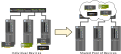
\includegraphics{pooling}
    \caption
    [Pooling internal devices increases flexibility and improves resource utilization and cluster performance]
    {If machines could pool their internal devices, it would be possible to avoid queuing work on dedicated machines with particular device configurations. Instead, each machine could dynamically compose the \gls{io} infrastructure needed to meet a workload's \gls{io} requirements, by borrowing devices from other machines and releasing them when they are no longer needed.}
    \label{fig:device-pool}
\end{figure}

Cluster computing applications often have high requirements to \gls{io} performance.
%
%For example, compute accelerators, such as \glspl{gpu} and \glspl{fpga}, are often used to increase the processing speed of computing tasks.
For example, many computing clusters rely on compute accelerators, such as \glspl{gpu} and \glspl{fpga}, to increase the processing speed.
%
In recent years, we have also seen a convergence of the high-performance computing, big~data, and machine~learning research fields.
%
This development has led to new demands to \gls{io} performance where fast access to high-volume storage devices is becoming a requirement for high-performance computing, while low latency networking and making use of compute accelerators have become cloud computing issues~\cite{Trivedi2011,Coates2013,Taherkordi2018}.
%
If \gls{io} resources~(devices) are scarcely distributed in the cluster, cluster machines with \gls{io} resources may become bottlenecks, for example when a workload requires heavy computation on \glspl{gpu} or fast access to storage.
%
Contrarily, over-provisioning machines with resources may lead to devices becoming underutilized if a workload's \gls{io} demands are more sporadic.
%
Distributed processing workloads may even require a heterogeneous cluster design, with widely different compositions of devices and memory resources for individual machines in the cluster.
%
Being able to share and partition devices between cluster machines at run-time leads to more efficient utilization, as individual machines may dynamically scale up or down \gls{io} resources based on current workload requirements (\cref{fig:device-pool}).



In order to meet the latency and throughput requirements of data-driven and compute-heavy workloads, there is a need for flexible, yet efficient, sharing of \gls{io} resources in a networked computing cluster.
%
This dissertation contributes to this goal by presenting a solution that enables distributing devices and sharing memory resources between machines interconnected with \gls{pcie}~\cite{spec:PCIe}.
%
By leveraging memory mapping functionality supported by the \gls{pcie} networking hardware, we make it possible to use resources residing in remote machines as if they were installed in the same machine.
%
Whether resources are local or remote is made transparent to application software, \gls{os}, and even device drivers, and remote resources can be used in a manner that is indistinguishable from using resources attached to the local \gls{pcie} bus.
%
Existing device drivers and application software may use remote resources without requiring any adaptations.
%
Not only does this make it easier to increase the overall resource utilization in the cluster, but it also becomes easier to design and implement distributed applications as software no longer needs to be written with accessing remote resources in mind,
but can instead be implemented as if all resources are local.
%
Using our solution, \gls{io} resources are no longer locked to individual machines, and memory and devices can be shared freely with other machines in the cluster.
%
Scaling out and using more hardware resources than there are available in a single machine becomes easier, and our solution improves both the performance of individual machines and the entire cluster as a whole.



\section{Background and motivation}\label{sec:motivation}
In cloud computing environments, dynamically scaling resources is often accomplished through virtualization. 
%
\Gls{vm} \glspl{hypervisor} may dynamically add virtual \gls{io} devices to \glspl{vminstance} on demand.
%
It is even possible to temporarily suspend computation to migrate \glspl{vm} to \glspl{hostmachine} with more hardware resources available, should the requirements of a \gls{vmguest} exceed the available local resources.
%
However, when the raw, bare-metal \gls{io} performance is required, for example in the case of \gls{gpu}-intensive machine~learning workloads, resource virtualization may not be a viable solution.
%
In this regard, it is possible to \lgls{passthrough}{``pass through''} physical \gls{io} devices to a \gls{vmguest} using an \gls{iommu}.
%
The \gls{iommu} facilitates direct access to hardware from the \gls{guest} without compromising the virtualized environment.
%
As such, \gls{passthrough} allows physical hardware to be used by a \gls{vmguest} with minimal software overhead.
%
However, as physical devices are tightly coupled with the \gls{host} they are installed in, this \gls{passthrough} technique suffers from a lack of flexibility.
%
Distributing \glspl{vm} across \glspl{host} in the network in a way that maximizes resource utilization and adapts dynamically to varying \gls{io} requirements, without sacrificing the bare-metal performance that pass-through provides, remains a challenge.



Another challenge is the networking technology itself. 
%
Despite having been a research topic for decades, moving data to remote computing units over a network remains a costly operation that introduces large performance overheads compared to using local resources.
%
As such, many \glspl{nic} support zero-copy of application memory from one system to another through \gls{rdma}~\cite{Huang2012}.
%
\Gls{rdma} is not only used in many distributed shared-memory cluster applications, but is also frequently used for implementing \gls{io} resource \gls{disaggregation} in software.
%
For example, \glspl{nvme} may be \gls{disaggregated} and shared with remote systems with very low latency.
This is the case for \gls{nvmeof}, where \gls{rdma} is used to provide direct access and avoid going through the block-layer of the \gls{os} on the server~\cite{Guz2018}.
%
Similarly, the result of a \gls{gpu} computation may be copied out of \gls{gpu} memory and onto the network directly using \gls{rdma}, without being copied to system memory first and going through the network stack~\cite{Venkatesh2014}.
%
However, while \gls{rdma} allows data to be transferred efficiently over the network, translation between the network protocol and the local \gls{io} bus is unavoidable. 
%
Compared to accessing a local device, this protocol translation incurs latency overheads that are not insignificant.
%
Moreover, as \gls{rdma} requires the use of specific programming models like message-passing~\cite{Jiang2004}, \gls{disaggregation} solutions based on \gls{rdma} are usually implemented either as application-specific \gls{middleware}, or as part of the application itself.
%
The sharing capabilities of \gls{rdma} solutions are, therefore, often limited to a single type of device.
Sharing several types of devices, for example both \glspl{gpu} and \glspl{nvme}, usually requires multiple \gls{disaggregation} implementations, and integrating them with each other may be a challenge.



\begin{figure}
    \centering
    \begin{subfigure}{\linewidth}
        \centering
        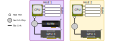
\includegraphics[width=.85\linewidth]{fabric-partitioning}
        \caption{Partitioning allows \glsfmtshortpl{cpu} and devices with different address domains to be isolated.}
    \end{subfigure}
    \par\vspace{5mm}
    \begin{subfigure}{\linewidth}
        \centering
        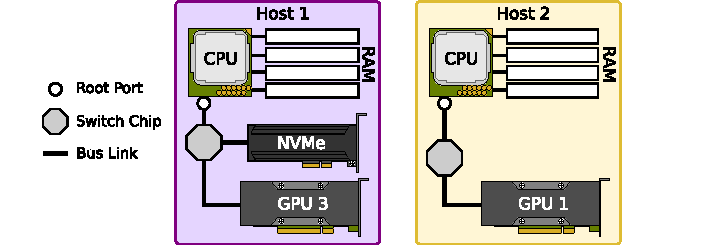
\includegraphics[width=.85\linewidth]{fabric-partitioning-device-tree}
        \caption{Machines have separate (logical) \glsfmtshort{pcie} device trees.}
    \end{subfigure}
    \caption[\Glsfmtshort{pcie} switch chips with partitioning support can be used to connect multiple \glsfmtshortpl{cpu} and freestanding devices to a common \glsfmtshort{pcie} fabric.]
    {\Glsxtrshort{pcie} switch chips with partitioning support can be used to connect multiple \glsxtrshortpl{cpu} and freestanding devices to a common \glsxtrshort{pcie} fabric. However, as systems are isolated, shared memory communication over \glsxtrshort{pcie} is not possible.}
  	\label{fig:partitioning}
\end{figure}



\begin{figure}
	\centering
    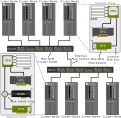
\includegraphics[width=.83\linewidth]{cluster-example}
    \caption[Example of a heterogeneous \glsfmtshort{pcie}-networked cluster with \glsfmtshort{ntb} adapter cards and external cables]{Example of a heterogeneous \glsxtrshort{pcie} cluster with external \glsxtrshort{pcie} links using adapter cards capable of \glsxtrshort{ntb}. The \glsxtrshortpl{cpu} as well as internal devices of all cluster machines~(nodes) are all attached to the same \glsxtrshort{pcie} network fabric.}
  	\label{fig:cluster-example}
\end{figure}



\begin{figure}
    \centering
    \begin{subfigure}{\linewidth}
        \centering
        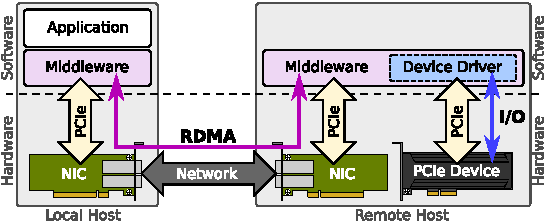
\includegraphics{direct-access-rdma}
        \caption{Accessing remote resources over traditional network using \glsxtrshort{rdma}.}
    \end{subfigure}
    \par\vspace{5mm}
    \begin{subfigure}{\linewidth}
        \centering
        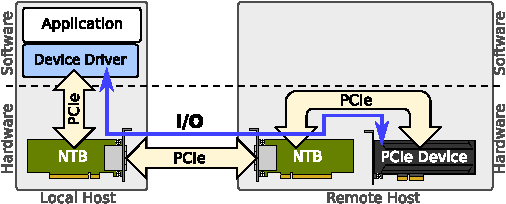
\includegraphics{direct-access-smartio}
        \caption{Accessing remote resources over native \glsxtrshort{pcie} using \glsxtrshort{ntb}.}
    \end{subfigure}
    \caption
    [Remote hardware can be accessed directly without any software in the critical path by using \glsfmtshortpl{ntb}]
    {Many distributed \gls{io} solutions have performance overheads because they rely on \gls{middleware} or other forms of software facilitation on the remote system. By setting up memory mappings through the \glsxtrshort{ntb}, remote hardware resources can be accessed directly without any software in the critical path.}
    \label{fig:direct-access}
\end{figure}



Extending the \gls{pcie} bus out of a single computer system and using it as a high-speed interconnection technology is a compelling alternative to distributed \gls{io} over a traditional network.
%
As \gls{pcie} is the standard for connecting \gls{io} devices to a local computer system, using only native \gls{pcie} would have clear performance advantage, since conversion between network protocol and \gls{io} bus would not be necessary~\cite{Fountain2005,Ravindran2008,whitepaper:Regula2004}.
%
However, since \gls{pcie} was originally designed to connect devices to the local \gls{cpu} on a motherboard, individual computer systems operate with different \gls{pcie} address domains.
%
Because of this, some \gls{pcie} switch chip hardware have virtualization support for dynamic partitioning~\cite{Chung2018,whitepaper:IDT,whitepaper:Microsemi,url:rackscale,url:liqid,url:gigaio}. 
%
Multiple \glspl{cpu} can be connected to the same \gls{pcie} fabric by mapping partitions to the individual address domains of each \gls{cpu}.
%
Additionally, devices can be attached directly to the partitionable switch chip, rather than being owned by individual machines.
%
This allows switch-attached devices to be logically assigned to different machines, as illustrated in \cref{fig:partitioning}.


Nonetheless, because partitioning isolates \glspl{cpu} in separate address domains, this approach does not make it possible for machines to share their \emph{internal} resources.
%
Memory, or other devices that are attached to the local \gls{pcie} bus and not the partitionable switch (chip), cannot be shared.
%
Thus, partitioning lacks the shared-memory capabilities needed to support host-to-host communication over native \gls{pcie}, and other networking technologies, such as Ethernet or InfiniBand, must be used instead.
%
Consequently, \gls{disaggregating} devices and sharing them with multiple machines at the same time require either alternative methods, like \gls{rdma}, or additional virtualization support in the device itself,~i.e., \gls{sriov}.
%Distributed applications must instead use other networking technologies to communicate, such as Ethernet or InfiniBand, 
%
While approaches using \gls{pcie} fabric partitioning can be said to enable a composable \gls{io} infrastructure~\cite{Chung2018}, they stop short of providing \emph{networking} capabilities over \gls{pcie}.



Due to its intrinsic memory addressing abilities and low latency overhead, it is desirable to use \gls{pcie} as the enabling networking technology for distributed, shared-memory communication~\cite{Shim2018,whitepaper:Regula2004,url:Meduri2011}.
%
This requires translating memory transactions from one machine's address domain to another.
%
By far, the most common way of translating addresses between different \gls{pcie} address domains is by using a special type of device called a \gls{ntb}~\cite{whitepaper:PLX,whitepaper:Regula2004,Hou2013,Tu2014}.
%
%\Glspl{ntb} can be embedded as a \gls{cpu} feature~\cite{whitepaper:Sullivan2010,url:LinuxNTB-AMD}, but are more commonly implemented in \gls{pcie} switch chips~\cite{whitepaper:PLX,pex8733}.
%
%Using such \gls{ntb}-capable switch chips to implement peripheral devices and cluster switches, it becomes possible to connect independent computer systems with plug-in host adapter cards and external cables, as depicted in \cref{fig:cluster-example}.
By using \glspl{ntb} to implement plug-in host adapter cards and cluster switches, it becomes possible to connect independent computer systems as depicted in \cref{fig:cluster-example}.
%
The memory address translation capabilities of \glspl{ntb} make it possible for a machine to map (parts of) the address space of remote systems.
%
Since all memory address translations are done in the \gls{ntb} hardware, memory-to-memory transfers are supported with very low latency~\cite{Lim2019,Tu2014}.



More interestingly, however, is the fact that in such \gls{ntb}-based networks, all \glspl{cpu} and internal \gls{pcie} devices are attached to the same, shared \gls{pcie} fabric.
%
Remote resources, such as the internal memory and devices of other machines, could be mapped into a local system and accessed through the \gls{ntb} with very little performance overhead.
%
Similarly, a device capable of \gls{dma} could also use the \gls{ntb} to access remote resources.
%
This approach eliminates the need to use memory on the remote system as an intermediate step when transferring data, and any software in the data transfer path can be avoided entirely, as shown in \cref{fig:direct-access}.
%
Rather than relying on dedicated servers or requiring that devices are attached to special switches, we could create distributed, peer-to-peer sharing system using \glspl{ntb};
%
\emph{all} machines in the cluster can share \emph{all} of their resources, including internal \gls{pcie} devices and system memory. 
%
Moreover, as centralized servers can be avoided, the risks of individual machines becoming performance bottlenecks or single points of failure are reduced.




However, setting up such \gls{ntb} mappings requires awareness of the address space on the remote system.
%
For example, a device driver must use addresses that correspond to the remote device's address space when initiating \gls{dma} transfers.
%
Extensive modifications to device driver software would be required in order to manage multiple address space layouts.
%
This is infeasible due to the vast amount of devices and device driver implementations that exist. 
%
Although we could use virtualization to hide the fact that devices are on the other side of an \gls{ntb}~\cite{Tu2013}, by relying on \glspl{vm} we would forgo the possibility of using bare-metal machines for processing.
%
Hence, a realistic solution based on \glspl{ntb} requires a mechanism for abstracting away the physical location of a resource, as well as the address space of the machine it is installed in, without requiring virtualization (although sharing to \glspl{vm} should \emph{also} be supported).

%However, setting up such \gls{ntb} mappings requires awareness of the address space on the remote system.
%%
%For example, a device driver must use addresses that correspond to the remote device's address space when initiating \gls{dma} transfers.
%%
%Hence, relying on \glspl{ntb} alone for enabling distributed \gls{io} and resource sharing is not a viable solution.
%%
%In order to manage multiple address space layouts, extensive modifications to existing device driver software would be required.
%%
%This is infeasible due to the vast amount of devices and device driver implementations that exist.
%%
%In this context, it is possible to use virtualization to mitigate the complexity of managing different \gls{pcie} address spaces.
%%
%The fact that devices are on the other side of an \gls{ntb} could be hidden for device drivers by distributing devices to \gls{vm} \glspl{guest} instead of physical \lgls{host}{host~machines}.
%%
%The \gls{hypervisor} on the host~machines can be modified to assist setting up necessary \gls{ntb} and \gls{iommu} mappings to the respective device memory and \gls{vm} memory, enabling \gls{passthrough} of remote devices to \gls{vm} \glspl{guest}~\cite{Tu2013}.
%%
%However, by relying on virtualization to hide complexity, this approach forgoes the possibility of using bare-metal machines for processing.
%%
%Even though \gls{passthrough} allows the device to be used directly by a device driver running in a \gls{guest}, requiring that compute tasks run in \glspl{vm} is a constraint that may add additional system load, as \gls{cpu} cycles are spent on \lgls{host}{hosting} the virtualized environment.
%%
%Another mechanism for using \glspl{ntb} while remaining agnostic about the address space in remote systems is therefore needed.
%%
%The physical location of a resource, as well as the address space layout in the machine it is installed in, must be abstracted away without requiring \glspl{vm} (but sharing resources to \glspl{vm} should \emph{also} be supported).



Nevertheless, this kind of abstraction gives rise to yet another challenge.
%
A device driver that is unaware that a device is remote may assume that the entire local address space can be reached by the device.
%
\Gls{ntb} maps must be in place \emph{before} the driver interacts with the device, but predicting in advance which memory addresses a device driver may use is generally not possible.
%
Deferring the action of mapping through the \gls{ntb} until a time when addresses may be known is not realistic, as this would require synchronizing with the remote system and introduce communication overhead in the performance-critical path.
%
A way to prepare the necessary memory-maps through the \gls{ntb}, without adding communication latency, is needed.

%Nevertheless, this kind of abstraction gives rise to another challenge. 
%%
%A device driver that is unaware that a device is remote may assume that the entire local address space can be reached by the device.
%%
%It is generally not possible to predict in advance which memory addresses a device driver may use, yet \gls{ntb} mappings must be in place before the driver initiates operations, such as \gls{dma} transfers.
%%
%Deferring the action of setting up these mappings until the device driver initiates \gls{dma}, or some other time when the specific addresses of \gls{dma} buffers may be known, is not realistic;
%%
%synchronizing with the remote system at this time will introduce communication overhead in the performance-critical path.
%%
%The naive solution is to map the entire system memory of all other machines in the cluster, but this workaround does not scale very well as the memory requirements will then increase for every machine added to the cluster.
%%
%A way to prepare the necessary memory-mappings through the \gls{ntb}, without adding additional communication latency, is required.




\section{Problem statement}\label{sec:problem}
Utilizing \gls{pcie} \glspl{ntb} to share resources among machines in a \gls{pcie}-networked cluster requires a mechanism for abstracting away the physical location of a resource, including the address space of the computer system it is installed in. 
%
More specifically, as it is desirable to avoid modifications to existing device drivers and application software, such a mechanism must also be able to present resources to the system as if they were locally installed.
%
This mechanism must also allow remote resources to be used with the same performance expected for native \gls{pcie},~i.e., with the same performance as if they were attached to the local \gls{pcie} bus.
%
Hence, the goal of this dissertation is to develop a framework for sharing and distributing \gls{io}~resources (devices and memory) in a way that eliminates the distinction between local and remote access of a resource. 
%
The challenges of this goal are addressed under the following research question: 
\begin{restatable}{question}{researchquestion}\label{question}
    Can \glspl{ntb} be leveraged to allow the internal memory and devices of individual computers in a \gls{pcie}-networked cluster to be shared with and used by remote machines in the cluster, as if these resources were local to the remote machines?
\end{restatable}
%
In particular, this research~question can be broken down into the following list of requirements that a solution must satisfy:


\begin{objective}\label{obj:distributed}
    Ubiquitous sharing in the cluster should be supported, allowing any machine to contribute any of its internal \gls{pcie} devices, and allowing any machine to be able to use shared devices, even contributing and using devices at the same time.
\end{objective}
The main motivation for our goal of building a system for \gls{io} resource sharing is to make it easier to scale out and use more resources than there are available in a single computer. 
If any standard \gls{pcie} device inside any machine could be shared with other machines, the \gls{io} resource utilization in the cluster could be greatly increased.
Additionally, by avoiding dedicated servers and allowing all computers in the cluster to participate in the sharing, contributing their own resources and using resources shared by others, we would effectively enable a distributed, peer-to-peer sharing model. 
This objective sets our goal apart from existing \gls{pcie}-based solutions, as these require a central server or devices that are directly attached to a \gls{pcie} switch.



\begin{objective}\label{obj:transparent}
    The fact that resources may be remote should be functionally transparent, allowing systems to use remote resources in the same way as if they were local, without requiring any modifications to device hardware, device drivers, host \gls{os}, or application software.
\end{objective}
If the solution could make remote devices behave as if they were locally installed, presenting resources to the system on a level ``underneath'' the \gls{os}, it would become possible to distribute devices to \emph{physical} hosts as well, and not only \glspl{vm}. 
In other words, remote resources should appear as if they were part of the local \gls{pcie} device tree, and application software could make use of remote devices using native interfaces in the same way it would use local devices.
%
Furthermore, by avoiding application- or device-specific \gls{middleware}, and instead memory-mapping remote system and device memory directly, existing device drivers and even the host \gls{os} itself would be able to interact with remote resources natively.
Avoiding any special adaptions to software would make scaling out significantly easier than what is currently possible with existing \gls{middleware}-based solutions for distributed \gls{io}, particularly those based on \gls{rdma}.



\begin{objective}\label{obj:performance}
    The fact that resources may be remote should be transparent with regard to performance, remote resources should be used with native \gls{pcie} performance, and as close to local access as possible.
\end{objective}
Moving data to remote units over the network introduces large performance overhead compared to accessing local resources. 
In order to further blur the hard separation between ``remote'' and ``local'', remote resources should not only behave functionally as if they were locally installed in the system using them, but also have comparable performance.
To achieve this, any communication overhead and intermediate data copying in the critical path must be completely avoided, a requirement that rules out (most) traditional methods of sharing resources over a network. 
Remote resources should be accessed directly over \emph{native} \gls{pcie}, which would improve the overall \gls{io} performance in the cluster.



\begin{objective}\label{obj:dynamic}
    Shared resources should be distributed \emph{dynamically}, and direct access to device memory and system memory should be configured at run-time, also between multiple devices residing in different hosts.
\end{objective}
As stated in \cref{obj:transparent}, the solution should work for physical hosts, and not only \glspl{vm}. Therefore, it must be possible to assign and reassign resources while all machines in the cluster are running, without requiring rebooting hosts or changing settings in the \gls{bios}.
For devices, this introduces the requirement that the \gls{os} supports hot-adding devices to the system (which most modern \gls{os} implementations do).
Not only would this would allow systems to dynamically scale up or down their \gls{io} resources based on immediate workload requirements, but devices could be more efficiently partitioned between machines in the cluster, increasing the overall resource utilization. 
Furthermore, the solution should also be able to automatically discover resource location, without requiring that the user knows anything about the underlying \gls{pcie} network topology, and dynamically set up memory mappings between devices, \glspl{cpu}, and memory resources. An example would be enabling \gls{pcie} \gls{p2p} between two or more \gls{dma}-capable devices that are physically installed in different machines.

    
\begin{objective}\label{obj:disaggregation}
    \Gls{disaggregation} of system memory, device memory, and device \emph{functionality} should be supported, and the solution should be able to distribute component parts to different hosts, as well as provide software facilities for resources that do not support \gls{disaggregation} in hardware.
\end{objective}
Because most device drivers are written in a way that assumes exclusive control over a device, some devices implement virtualization support in hardware,~i.e., \gls{sriov}, that makes them appear to a system as having multiple \glspl{vf}. 
%
The solution should be able to \gls{disaggregate} such \gls{sriov}-capable devices, and distribute their \glspl{vf} to different machines, allowing multiple computers to use the same device simultaneously.
%
However, since not all devices implement \gls{sriov}, the solution should also provide a device driver \gls{api} that will make it possible to \gls{disaggregate} memory and device resources in software.
%
In addition to the native sharing capabilities described in \cref{obj:distributed,obj:transparent,obj:performance,obj:dynamic}, this \gls{api} 
would provide facilities for memory-mapping device registers as well as mapping shared memory segments for a \gls{dma}-capable device.
%
Effectively, this would bring shared-memory concepts to device driver implementations, allowing device operation and device resources to become part of the same global address space as distributed cluster applications.
%
This would allow multiple machines to simultaneously share the same, non-\gls{sriov} device, as well as making it possible to combine traditional \gls{io} with \gls{pcie} cluster capabilities such as zero-copy data transfer and multicasting.
%
Moreover, the \gls{api} should be designed so that a driver implementation does not need to consider the system-local address space of the computer system where a device is installed, thus alleviating the complexity of programming device drivers for remote devices using \glspl{ntb}.



\begin{objective}\label{obj:experiments}
    To prove real-world deployment capabilities, the solution should be tested on realistic and relevant workloads and benchmarks.
\end{objective}
In order to confirm that \gls{io} resources can be distributed to, and shared with, remote machines, a comprehensive performance evaluation covering all components of the implementation is needed.
%
As the solution should provide \emph{native} \gls{pcie} performance (\cref{obj:performance}), all parts should be thoroughly tested with latency and throughput in mind, in order to reveal any potential performance bottlenecks.
Standardized test suites should be used as far as possible, to prove that application software really can be unmodified (\cref{obj:transparent}).
%
Moreover, to demonstrate the completeness of the solution, the evaluation should also include workloads relying on different \gls{pcie} network topologies and include several types of devices, such as \glspl{nvme}, \glspl{gpu}, and \glspl{nic}.
%
Finally, a prototype device driver using the device driver \gls{api} (\cref{obj:disaggregation}) should be developed and evaluated. This driver should demonstrate that it is possible to \gls{disaggregate} a non-\gls{sriov} device in software, and shared with multiple machines simultaneously. 
%
The driver should also demonstrate how it can rely on memory \gls{disaggregation} and shared memory capabilities to implement data path optimizations.



\section{Scope and limitations}\label{sec:scope}
The research presented in this dissertation contributed to a collaborative project between academia and industry, with Dolphin Interconnect Solutions~(Dolphin) as the industry partner.\footnote{Funded by the Research Council of Norway under the ``Unified PCI Express for Distributed Component Virtualization'' project (RCN/NFR \#235530), with additional contributions from the ``LADIO: Live Action Data Input/Output'' project (EU H2020 \#731970).}
%
The goal of this project was to develop a new framework for sharing devices and memory resources among computer systems connected with \gls{pcie}.
%
The scope of this dissertation is the implementation and performance evaluation of the fundamental mechanisms that make this framework possible: \textbf{the discovery, addressing, access, and use of remote \gls{pcie}-attached resources}.
%
We aim to support this for three different abstraction levels:
\begin{enumerate}
    \item Dynamically distributing devices to remote machines.
    \item Dynamically distributing (physical) devices to \glspl{vm} running on remote machines.
    \item Enabling \gls{disaggregation} of devices and memory resources in software, allowing them to be shared \emph{simultaneously} by software processes running on several machines simultaneously.
\end{enumerate}



Exploring resource sharing possibilities using alternative networking technologies, such as InfiniBand, is outside the scope of our dissertation.
%
The desired objectives for the sharing framework, as stated in \cref{sec:problem}, necessitate the use of \gls{pcie} \glspl{ntb}. %due to their shared-memory nature and performance requirements.
%
Dolphin's \gls{ntb} adapter cards and cluster switches make it possible to build heterogeneous computing clusters in various network topologies.
%
\Cref{fig:cluster-example} is an example of such a cluster.
%
Memory mappings between machines are configured using Dolphin's existing \gls{ntb} driver, and application software may use the \gls{sisci} programming \gls{api} to interact with this \gls{ntb} driver in order to dynamically set up and tear down these memory mappings and implement shared-memory communication.
%
In order to fit our work into this existing cluster networking foundation, we rely on Dolphin's \gls{ntb} hardware and have implemented our sharing framework as part of their driver stack.
%
This makes it possible to extend existing functionality, rather than developing an entirely new \gls{ntb} driver from scratch.
%
To enable software \gls{disaggregation}, for example, we can add device-oriented semantics and device driver support functions to the already existing \gls{sisciapi}. 
%, instead of requiring that cluster application software must convert and translate and between different \glspl{api}.
%
Even so, it should be pointed out that while our specific implementation is building on Dolphin \glspl{ntb}, the ideas and concepts of our work are general, and can in fact be implemented for \emph{any} \gls{ntb} hardware that has similar capabilities.



Using our framework, both \gls{host}~machines and \glspl{vm} should be able to use shared devices.
%
In order to accomplish this, resources must to be presented to the system at the \gls{os}-level so that interactions with a device can be intercepted. 
%
This intercepting mechanism involves manipulation of device driver interfaces and requires a detailed understanding of \gls{os} internals.
%
For this reason, our framework is implemented for Linux, as its source code is available as open source and may be studied.
%
For the same reason, we have also extended the \gls{kvm} in order to support sharing devices with \glspl{vmguest}.
%
Regardless, we do not limit our work to a specific Linux distribution, as it is possible to support several different versions of the Linux kernel.
%
Note that for \glspl{vm}, there are no limitations for which \gls{os} may run in the \gls{guest}.



As per \cref{obj:distributed}, sharing of any \gls{pcie} device should be supported, from \gls{pcie}~1.0 devices up to \gls{pcie}~4.0 devices.
%
Our evaluation includes a wide range of common (and commodity) devices, like \glspl{nvme}, Ethernet~\glspl{nic}, and \glspl{gpu}.
%
However, the framework should also not require any modifications to existing device driver implementations or device hardware~(\cref{obj:transparent}).
%
While \gls{ntb} clusters can be anywhere from 2 up to 60~machines, in many different network topologies, a limitation of the evaluation of our implementation is that it for the most part includes scenarios with cluster networks of only a few machines, since devices can only be used by one machine at the time.
%
Nevertheless, more advanced network topologies and larger clusters (of up to 60~machines) are used in a few experiments, as our framework supports \gls{disaggregating} devices in software, allowing devices to be used simultaneously by many machines.



Finally, it should be mentioned that several related research topics emerge from enabling the envisioned sharing framework this dissertation aims for.
%
Examples include finding algorithms for scheduling workloads on different machines in the cluster in order to optimize resource utilization, or choosing the appropriate trade-off between fairness and workload performance requirements when provisioning resources to machines.
%
The security implications of allowing remote machines to use and control internal system resources is also something that becomes relevant in the context of this sharing framework.
%
A ``finished product'' should attempt to address most of these topics, and ideally include tools and services for managing resources and orchestrating workloads on the cluster level.
%
However, we consider this to be outside the scope of this dissertation, and we only focus on the fundamental mechanisms that enable the low-level sharing functionality.



\section{Research methodology}\label{sec:methodology}
Choosing an appropriate research methodology for problems in computer~science is challenging.
%
Many methodologies come with their own set of considerations and potential pitfalls~\cite{McGrath1981}.
%
Finding a methodology is not made easier by the fact that computer~scientists themselves do not seem to agree on the age-old philosophical question of whether computer~science should be considered applied mathematics, engineering, or a science~\cite{Denning2005}.


According to Eden~\cite{Eden2007}, computer~science as a discipline can broadly be divided into three different research paradigms:
\begin{itemize}
    \item The rationalist paradigm, which defines computer~science as a branch of mathematics. 
        The paradigm seeks certain, a~priori knowledge of systems or processes through means of deductive reasoning.
    \item The technocratic paradigm, which defines computer~science as an engineering discipline.
        The paradigm seeks probable, a~posteriori knowledge about systems or processes through implementation (or prototyping) and empirical validation in the form of testing.
    \item The scientific paradigm, which defines computer~science as a natural (empirical) science.
        The paradigm seeks both a~priori and a~posteriori knowledge about systems or processes by combining formal deduction and scientific experimentation.
\end{itemize}
Note that the technocratic concept of a ``test'' differs from scientific experiments, in that the purpose of the former is to establish to which extent a set of requirements are met, whereas the latter is designed to corroborate or refute a hypothesis.
%%
If a test fails (to meet a requirement), the implementation must be revised. 
%
If an scientific experiment ``fails'', it is the theory (or understanding) that must be revised instead.


An almost identical classification of paradigms is given by the ACM Task Force on the Core of Computer Science~\cite{Comer1989}.\footnote{ACM use the names ``theory'', ``design'', and ``abstraction'' for these paradigms instead.}
%
They additionally note that the three paradigms are intrinsically intertwined, as computer~science is both deeply rooted in mathematics and has its own theory, experimental method, and engineering---in contrast to most physical sciences, where the engineering disciplines that apply their findings are considered separate disciplines.
%
The three paradigms are therefore equally fundamental to computer~science.



The subject matter of this dissertation touches on several sub-areas of computer~science, including computer and hardware architecture, distributed computing, \gls{os} fundamentals, and communication networks.
%
While all three paradigms can be applied to these sub-areas~\cite{Comer1989}, it is the technocratic paradigm which lends itself best to answering the overall problem~statement of this dissertation~(\cref{sec:problem}).
%
Neither the rationalist nor the scientific paradigm are particularly well-suited.
%
It is unrealistic to make a model through a~priori knowledge alone, due to the complexity of the many different hardware and software components of real-world computer systems.
%
Similarly, the process of gathering data with the goal of understanding the behavior of an indeterministic system, in order to create a statistical model and make predictions about it, seems equally unfit in this context.



As many solutions for distributed \gls{io} already exist, the motivation for this dissertation is not simply to make it easier for machines to share resources efficiently, but to do so by using a new approach altogether:
%
we attempt to unify traditional device \gls{io} with distributed, shared-memory computing by utilizing the inherent memory mapping capabilities of \glspl{ntb}.
%
It is desirable to realize this approach by \textbf{building a working prototype}, in order to explore potential opportunities and weaknesses along the way.
%
As such, we follow the technocratic paradigm of iteratively designing, implementing, and testing a solution according to the objectives given in \cref{sec:problem}:
%
\begin{itemize}
    \item 
        A mechanism must be developed to make remote resources appear and behave exactly as if they were part of the local \gls{pcie} tree.
        %
        In order to not require any special adaptions of existing hardware, device drivers, or application software, this mechanism must be completely transparent.
        %
        This mechanism must also be thoroughly tested using a wide range of functionality tests, for many different types of devices and device driver implementations.
        %
        As we make a point of using unmodified hardware and software, commodity devices and widely available software, such as standard benchmarking tools and well-known applications, should be used in the validation of our solution.
        %
        A complete functionality evaluation should also include a variety of different cluster network topologies and machine configurations, including \glspl{vm}.

    \item 
        A wide range of latency and throughput benchmarks should be used to measure the performance of the critical \gls{io} data path.
        %
        Since the solution allows machines to use the internal devices and memory in other (remote) machines as if these resources were locally installed, it is possible to rely on comparison testing.
        %
        Tests looking at individual \gls{io} operations, such as reading/writing to an \gls{nvme} or copying memory out of \gls{gpu} memory, can first be performed using local resources (without our solution) to establish a performance baseline.
        %
        Then, the tests can repeated for remote resources using our solution, allowing us to compare the results and subsequently identify which component of the solution that needs to be improved.
        %
        Note that the different iterations and gradual improvements of our solution can be seen in \crefrange{paper:nossdav}{paper:tocs}.

    \item 
        Our implementation process should also identify and explore new possibilities that are enabled by the solution.
        %
        The strength of our shared-memory approach is best highlighted by demonstrating capabilities that other resource sharing solutions lack.
        %
        For instance, as CUDA unified memory~\cite{url:unified-memory} can be supported by our solution, even for \glspl{gpu} that reside in \emph{different machines}, we should perform experiments with direct memory-to-memory transfers across the cluster network.
        %
        Other possibilities, such as exploiting memory \gls{disaggregation} to implement memory locality optimizations or using \gls{pcie} \gls{multicasting} to replicate data across several machines in a single operation, should also be explored.
        %
        We should not only investigate how different cluster network topologies affect the data path, but we should also prove the flexibility of our solution and demonstrate several of the sharing scenarios that are made possible.

    \item
        A realistic and \gls{io}-intensive computing task, for example involving machine~learning, should be used to put the solution under heavy load.
        %
        By running a real-world application using several \gls{io} resources, we can observe the accumulated effects of any performance overhead caused by the implementation that are not visible on their own.
        %
        Moreover, this kind of stress testing also proves that the solution is stable and gives reliable performance for repeated runs, and that it does not have any unintentional side-effects that affect systems over time.
        %
        Finally, showing that the solution works for a realistic workload has the additional purpose of proving that scaling real-world applications is possible.

\end{itemize}
%
For the sake of convenience, functionality testing and the overall validation process is implicit in the performance experiments presented in this dissertation.
%
It should also be noted that while the presented experiments primarily use Intel~Xeon as the \gls{cpu} architecture and \glspl{nvme}, Ethernet~\glspl{nic}, and Nvidia \glspl{gpu} were used for shared resources, we also used additional \gls{cpu} architectures and devices during the development and validation phases.
%
This includes \gls{cpu} architectures like AMD and ARM, and other devices like \glspl{fpga}, sound cards, and \gls{pcie}-attached cameras.


\section{Contributions}
This dissertation contributes to the topic of resource sharing and distributed \gls{io} facilitation in cluster computing systems, and has been presented in five peer-reviewed venues: two conference workshop publications, one short-length demonstration paper, and two journal articles.
These publications are included as \crefrange{paper:nossdav}{paper:tocs} and contain the bulk of the implementation details, particularly \cref{paper:tocs}, which presents the entire solution as a whole.

We have developed a framework called \emph{SmartIO} for sharing resources and distributing devices in a heterogeneous, \gls{pcie}-networked cluster.
%
In particular, the main contributions of this dissertation are listed as follows:
\begin{itemize}
    \item Testing and evaluation of the \emph{Device~Lending} mechanism for \textbf{distributing \gls{pcie} devices to remote systems} (see \cref{paper:nossdav,paper:mmsys}): 
        %
        using Device~Lending, any standard \gls{pcie} device, such as \glspl{nvme}, \glspl{gpu}, \glspl{nic}, and \glspl{fpga}, may be assigned to a remote system. 
        %
        The device appears to the remote system as if it has been dynamically hot-added to the system, allowing existing device drivers to use the device without requiring any modifications to software.

    \item Implementation of a \textbf{new mechanism for distributing devices to \glspl{vm}} running on any host machine in the cluster (see \cref{paper:srmpds,paper:cc}): 
        %
        we have developed an extension to the \gls{kvm} based on the \emph{\gls{mdev}} interface, enabling direct access to remote physical hardware devices for \glspl{vmguest} and setting up memory mappings for the devices. 
        %
        This \gls{mdev} implementation includes a method for dynamically discovering \gls{guest}-physical memory layout. Using this \gls{mdev} extension, local and remote devices can be \lgls{passthrough}{``passed through''} to \glspl{vm} and used with bare-metal performance.
	
    \item Improvement of the Device~Lending and \gls{kvm}/\gls{mdev} mechanisms by implementing \textbf{support for multiple devices} and \textbf{supporting devices in different physical machines} (see \cref{paper:srmpds,paper:cc}):
        %
        a method for resolving device memory addresses and setting up memory mappings, in a way that is transparent to both the devices and the device drivers, is implemented. 
        %
        This enables direct data transfers between multiple devices without violating the principle of making devices appear local to the system(s) using them.

    \item Extension of the \gls{sisci} shared-memory \gls{api} with new, \textbf{device-oriented programming semantics and support functions for writing device drivers as shared-memory applications} (see \cref{paper:tocs}):
    %
	this \gls{api} extension makes it possible to \gls{disaggregate} devices and device memory in software, similarly to \gls{rdma} \gls{disaggregation} solutions.
    %
	Unlike \gls{rdma} solutions, however, remote resources can be memory-mapped directly into the virtual address space of a software process.
	%
	Through our \gls{api} extension, device driver implementations may take full advantage of \gls{pcie} shared memory capabilities, such as remote memory access and multicasting, without requiring awareness of the underlying \gls{pcie} topology and the different address domains of remote systems.
	%
	This makes it easier to optimize data flow through the \gls{pcie} network, as software no longer needs to be written with accessing remote resources in mind, but can be implemented as if resources are local.

    \item Development of a \textbf{new prototype \gls{nvme} device driver}\footnote{The prototype \gls{nvme} device driver is open source and can be found at \mbox{\url{https://github.com/enfiskutensykkel/ssd-gpu-dma}}} using our device-oriented \gls{api} extension (see \cref{paper:tocs}):
        although the Device~Lending mechanism and \gls{mdev} extension make it possible to use existing device drivers, most device drivers are written in a way that assumes exclusive control over the device. Therefore, a distributed device (\gls{function}) may only be used by a single user at the time.
        %
    To demonstrate software-enabled \gls{disaggregation}, we have implemented a \emph{distributed} \gls{nvme} driver. 
    %
    As a proof of concept, we show that a single NVMe device can be shared and operated by multiple cluster machines simultaneously, without requiring \gls{sriov}.
	This driver also demonstrates how multiple sharing aspects of SmartIO may be combined, 
	by \gls{disaggregating} remote GPU memory and enabling memory access optimizations.

    \item A \textbf{comprehensive performance evaluation} covering all parts of SmartIO and the implementation of performance optimizations (see \cref{paper:mmsys,paper:cc,paper:tocs}):
        %
        with the goal of not incurring any performance overhead beyond that of native \gls{pcie}, the performance of using remote resources with SmartIO is comparable to that of local access (in terms of latency and throughput).
        %
        To prove that SmartIO is a viable and efficient solution for \gls{io} resource sharing also for realistic scenarios, two different image classification workloads relying on multiple \glspl{gpu} and \gls{nvme} storage have also been tested.
	
\end{itemize}
%
Finally, it should be noted that the research of this dissertation has had impact on real systems, as several components of SmartIO have already been incorporated into the product line of Dolphin Interconnect Solutions, and others are currently being adapted for real-world deployment.\footnote{{\url{https://www.dolphinics.com/solutions/pcie_smart_io.html}}}


\section{Outline}
This dissertation describes the design, implementation, and evaluation of the SmartIO framework for efficient sharing of resources between \gls{pcie}-networked computers.
%
The complete framework is described in detail in \cref{paper:tocs}, with the individual components and parts explained in \cref{paper:nossdav,paper:srmpds,paper:cc}.
%
Additionally, these papers show the evolution towards the complete framework, including different iterations of the framework components and gradual performance improvements.
%
The rest of this dissertation is organized as follows:
%
\begin{description}
    \item[\cref{chapter:smartio}]
        gives a brief summary of SmartIO.
        %
        We describe the initial idea and challenges for SmartIO, and provide a high-level overview of the implementation.
        %
        We also present related work focused on \gls{io} resource sharing in cluster networks.

    \item[\cref{chapter:conclusion}]
        summarizes our work and presents candidates for future work.

    \item[\cref{paper:nossdav}]
        describes the initial implementation of the Device~Lending component of SmartIO.
        %
        We evaluate how performance is improved by using Device~Lending to enable \gls{dma} transfers directly between a \gls{gpu} and remote memory, compared to using \gls{rdma} to achieve the same.

    \item[\cref{paper:mmsys}]
        is a demonstration of how the Device~Lending component can be used for a realistic video stream processing workload implemented for \glspl{gpu}.
        We demonstrate how real-time processing requirements can be met by using Device~Lending to scale up the number of available \glspl{gpu}.

    \item[\cref{paper:srmpds}]
        presents the \gls{mdev} component of SmartIO and how we improved the initial Device~Lending implementation with support for multiple devices residing in different machines. 
        %
        We evaluate how performance is improved by enabling \gls{p2p} \gls{dma} transfers directly between devices instead of needing to bounce data transfers via system memory, and also identify performance issues with relying on the \gls{iommu}.

    \item[\cref{paper:cc}]
        is an extension of \cref{paper:srmpds} and provides an extended evaluation of both \gls{mdev} and Device~Lending.
        %
        We show how different cluster network topologies affect \gls{dma} performance, for both \glspl{hostmachine} and \glspl{vmguest}.
        %
        Additionally, we also describe how we improved the original \gls{mdev} component with a mechanism for detecting \gls{guest}-physical memory layout.

    \item[\cref{paper:tocs}]
        presents the entire SmartIO solution as a whole, including the final iterations of the Device~Lending and \gls{mdev} components.
        %
        We also introduce the \gls{sisciapi} extension that makes it possible to \gls{disaggregate} devices and memory resources in software.
        %
        A thorough and complete performance evaluation of all parts and components of SmartIO is provided, in order to prove that the final implementation does not cause \emph{any} performance overhead compared to native \gls{pcie}.
\end{description}


	\chapter{SmartIO}\label{chapter:smartio}
SmartIO is a solution for allowing the local resources of a machine,~i.e., memory and devices, to be shared with and used by remote machines, over standard \gls{pcie}.
%
Our solution works for \emph{all} standard \gls{pcie} devices and their Linux device drivers, no special adaptation is needed in either hardware or software to make this sharing possible.
%
SmartIO is fully distributed and avoids dedicated servers.
%
All machines in the cluster~network may contribute their own local resources and access remote resources.
%
Furthermore, as remote devices and memory resources are accessed over native \gls{pcie}, they can be shared and used by remote machines with very low latency and extremely low computing overhead.
%
Whether devices are actually local or remote becomes irrelevant to the user, as SmartIO eliminates this distinction, with regard to both functionality and performance.
%
In other words, SmartIO is a flexible and efficient solution for scaling out and using more hardware resources than there are available in a single machine.


\section{Underlying idea}\label{sec:idea}
\begin{figure}
    \centering
    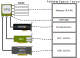
\includegraphics{bus-enumeration}
    \caption[Devices are mapped to the same address space as the \glsfmtshort{cpu} and system memory]
    {Device memory regions (\glsxtrshortpl{bar}) are mapped to the same address space as \glsxtrshort{cpu} and system memory, allowing
    the \gls{cpu} to read from and write to device memory the same way it would access \glsxtrshort{ram}. Devices can similarly use \gls{dma} to read from and write to \glsxtrshort{ram}.}
    \label{fig:bus-enumeration}
\end{figure}
The defining feature of \gls{pcie}~\cite{spec:PCIe} is that devices are mapped into the same address space as the \gls{cpu} and \gls{ram}, as seen in \cref{fig:bus-enumeration}.
%
This allows a \gls{cpu} to read from and write to device memory in the same manner it would access \gls{ram}, also known as \gls{mmio}.
%
Likewise, devices capable of \gls{dma} may read from and write to \gls{ram} directly.
%
\Gls{pcie} also uses \gls{msi}, allowing devices to raise interrupts by writing to an address reserved by the \gls{cpu} instead of requiring dedicated interrupt lines.



This address space mapping occurs when a system enumerates the \gls{pcie} bus and accesses the \gls{cfgspace} of each device.
%
A \gls{cfgspace} contains a description of the capabilities of a device, such as its memory regions.
%
The system will reserve a memory address range for each of these device memory regions, and by writing the start address of these regions to the device's \glspl{bar}, a device is made aware of the address space mapping.
%
Therefore, the term ``\gls{bar}'' is used interchangeably for a region of device memory.
%
Addresses reserved by the system for interrupts are also written to the device's \gls{cfgspace}.
%
For more details on \gls{pcie}, particularly how memory transactions are routed, please refer to \paperref{tocs:pcie,cc:pcie}.



\begin{figure}
    \centering
    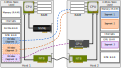
\includegraphics[width=.99\textwidth]{ntb-example}
    \caption[Two computer systems connected using \glsfmtshortpl{ntb}, and the \glsfmtshortpl{ntb} translate between the two different address domains]
    {Two computer systems connected together using \glspl{ntb} and external cables. Host~1 has mapped \glspl{segment} of Host~2's memory through its local \gls{ntb}, providing Host~1 with ``windows'' into the remote system's address space. The \glspl{ntb} translate addresses between the two independent address spaces.}
    \label{fig:ntb-example}
\end{figure}



As depicted in \cref{fig:ntb-example}, it is possible to connect computer systems with different address spaces together over \gls{pcie} by using \glspl{ntb}.
%
\Glspl{ntb} can be embedded as a \gls{cpu} feature~\cite{whitepaper:Sullivan2010,url:LinuxNTB-AMD}, but are more commonly implemented in \gls{pcie} switch chips~\cite{whitepaper:PLX,pex8733}.
%
By using such \gls{ntb}-capable switch chips to implement peripheral devices, independent computer systems can connect with plug-in host adapter cards and external cables.
%
To the system, the \gls{ntb} appears as a normal \gls{pcie} device\footnote{The \gls{pcie} terminology for individual \glspl{devicefunction} is ``\glspl{ep}''. We use the terms ``device'' and ``\gls{function}'' as synonyms for a \gls{pcie} \gls{ep} throughout this dissertation.} with one or more \glspl{bar} that are reserved and mapped during the enumeration process.
%
However, rather than being backed by device registers or device memory, the \gls{ntb} instead forwards reads and writes to its \glspl{bar} from one side of the \gls{ntb} to the other, translating memory addresses in the process.
%
The \gls{ntb} uses a \gls{lut} for address translation, which can be configured dynamically during run-time.
%
By using different base offsets in this \gls{lut}, it is possible to configure several memory-mappings (or ``windows'') into the address space of a remote system.
%
\Cref{fig:ntb-example} illustrates how arbitrary memory addresses on the remote system can be mapped, allowing the local \gls{cpu} to access remote memory as if it was local device memory.
%
Although address translation between the different address spaces is very fast since the \gls{lut} is implemented in \gls{ntb} hardware, the number of \gls{ntb} windows is limited by the maximum number of table entries.
%
More details on how \glspl{ntb} work can be found in \paperref{tocs:pcie-ntb}.



Since device memory on a remote system is part of the same address space as system memory, we can use an \gls{ntb} to map memory of a remote device.
%
We show this in \cref{fig:ntb-example}, where Segment~3 is allocated in \gls{gpu} memory rather than system~\gls{ram}, but still mapped for the \gls{cpu} of Host~1's similarly to the other \glspl{segment}.
%
By mapping all \glspl{bar} of a remote device for a local \gls{cpu}, it would be possible to perform memory operations on the remote device, such as reading from or writing to device registers.
%
Moreover, device~\gls{dma} is not limited to reading and writing to system \gls{ram}, but can also be used to access memory on other devices in the same address space.
%
This is known as ``\gls{p2p}'' in \gls{pcie}, and provides us with an opportunity as it becomes possible for a device to read and write directly across an \gls{ntb}.
%
We can use this to map memory resources for a device, be it \gls{ram} or memory of other devices. 
%
Furthermore, because \gls{pcie} uses \gls{msi}, it is even possible to map interrupt addresses through an \gls{ntb}, as they too are mappable.




\section{Main challenges}\label{sec:challenges}
Although \glspl{ntb} provide the fundamental memory mapping capabilities that can facilitate the use of remote devices, the challenge is to avoid requiring that device drivers must be aware of remote-side address spaces.
%
As touched upon in \cref{sec:motivation}, this is desirable in order to use existing device driver implementations.
%
For a device driver running on a local~machine to be able to use a remote~device, we must make sure that the driver uses addresses that is mapped through both the local and remote \glspl{ntb}.
%
For instance, when the device driver attempts to access \glspl{devicebar}, we must make sure that the driver uses memory addresses that are mapped through the \gls{cpu}-side \gls{ntb} without the driver or device being aware of this.
%
Conversely, when the device driver attempts to initiate \gls{dma} transfers or configures an interrupt vector address, we must find a way to transparently inject memory addresses that are mapped through the remote, or device-side, \gls{ntb}.



One possibility is to use virtualization to mitigate the complexity of managing different address spaces.
%
The fact that devices are on the other side of an \gls{ntb} could be hidden for device drivers by distributing devices to \gls{vm} \glspl{guest} instead of physical \lgls{host}{host~machines}, for example with \gls{passthrough}.
%
However, while \gls{passthrough} allows devices to be used by \glspl{vmguest} directly, \emph{requiring} that compute tasks run in \glspl{vm} will limit the generality of a solution.
%
Virtualization is not necessarily appropriate in all circumstances, as \gls{cpu} cycles are spent on \lgls{host}{hosting} the virtualized environment, thus adding additional system load.
%
Instead, a more general mechanism is needed for abstracting away the complexity of dealing with a remote-side address space.
%
This mechanism must support abstracting remote address spaces for \glspl{vm} and bare-metal machines alike.



\Gls{dma} is particularly challenging in this context.
%
A device driver running on the \gls{hostmachine} may assume that any local memory address can be reached by the device, but as explained in \cref{sec:idea}, the \gls{ntb} only provide \emph{windows} into a remote address space.
%
It is generally not possible to predict in advance which memory addresses a device driver may use, yet memory must be mapped through the \gls{ntb} before the driver, unaware that the device is remote, initiates \gls{dma} transfers.
%
Deferring the action of mapping memory through the \gls{ntb} until a device driver initiates \gls{dma}, or some other time when the specific addresses of \gls{dma} buffers and \gls{vm} memory can be known, is not viable;
%
synchronizing with the remote system at this time will introduce communication overhead in the performance-critical path.
%
The naive solution is to map the entire system memory for the device, but this workaround requires the \gls{ntb}~\glspl{bar} to be at least \emph{as large} as the size of \gls{ram}.
%
This does not scale very well, as it would effectively limit the number of machines the cluster can support.
%
Each new machine using a device would increase the device-side \gls{ntb} memory requirements by its entire \gls{ram} size.
%
Moreover, as the number of maps supported by an \gls{ntb} is also limited (by the size of its \gls{lut}), it is crucial to conserve memory maps wherever possible.
%
We must find a way to prepare memory-maps through the \gls{ntb} in advance of use, in order to avoid adding communication latency in the critical path, and without requiring that the entire memory is mapped for the device.



The challenge of \gls{dma} transfers is compounded for \gls{vmpassthrough}.
%
\Gls{passthrough} is possible by using the \gls{iommu} to create a virtual \gls{io} address space for a device that corresponds to the virtual address space of the \gls{vm}~\cite{url:LinuxVFIO,url:LinuxIOMMU,Muli2006}, also known as the ``\gls{guestphys} address space''.
%
For \gls{passthrough} of a local device, this makes it possible for the device driver running in the \gls{vmguest} to use any (virtualized) memory address when initiating \gls{dma} transfers.
%
In our case, however, the driver must use addresses that are mapped through the \gls{ntb} in order for a remote device to reach local \gls{hostphys} memory.
%
In order to support \gls{passthrough}, we must devise a method for mapping the physical memory backing the \gls{vmemulator} through the \gls{ntb}, using device-side \gls{io} addresses that mirrors the \gls{guestphys} address space.



The published papers provide further details on the challenges facing our solution as part of the description of the implementation of the different components of SmartIO.
%
Particularly \paperref{tocs:lending,tocs:mdev,tocs:nvme} provide a more in-depth explanation of what the main challenges are, and they also explain how SmartIO tackle them.
%
A discussion of additional considerations is given in \paperref{tocs:disc}.



\section{Implementation}\label{sec:implementation}
In our framework, computer systems act as \emph{``\glspl{borrower}''} and \emph{``\glspl{lender}''}.
%
A \gls{lender} is a computer system that registers one or more of its internal \gls{pcie} devices with SmartIO, allowing these devices to be distributed to and used by remote machines.
%
A \gls{borrower} is a system that is currently using such a device. 
%
While a device only has one \gls{lender}, namely the computer system where it is physically installed, there can be several \glspl{borrower} using it simultaneously.
%
SmartIO also makes it possible for a system to act as both \gls{lender} and \gls{borrower} at the same time, lending out its own local devices and simultaneously borrowing remote devices from other machines.



Basing our framework on standard \gls{pcie} is a a crucial part of the design.
%
Not only does this allow commodity devices to be operated remotely by standard device drivers over native \gls{pcie}, but this design also means that the implementation complexity of SmartIO lies entirely in software.
%
In fact, SmartIO can be implemented for existing computer systems that are connected using \glspl{ntb} in any network topology, regardless of whether the \glspl{ntb} are switch chips soldered onto a motherboard or implemented as plug-in adapter cards.



Unlike other solutions for distributed \gls{io}, SmartIO combines traditional \gls{io} with distributed shared-memory functionality in a seamless manner.
%
Sharing is supported at multiple abstraction levels:
%
devices may be distributed to physical \glspl{hostmachine} and to \glspl{vm} alike.
%
Individual \lgls{function}{device functions} of \lgls{function}{multi-function} devices may be distributed to different machines in the network, or to the same machine should it require multiple resources.
%
SmartIO also provides software facilities for \gls{disaggregating} devices and memory resources, allowing device drivers to be implemented as part of distributed cluster applications or other \gls{userspace} applications. 
%
This makes it possible for several machines to simultaneously share a single \lgls{function}{device~(function)}.
%
It is even possible to \emph{combine} the sharing methods of SmartIO. 
%
For example, we can \gls{disaggregate} the device memory of a remote \gls{gpu} using the \gls{apiext} while it is being borrowed through \gls{dl}, or we can share \glspl{vf} of an \gls{sriov} \gls{nic} with both physical \glspl{hostmachine} and \glspl{vm}.


\begin{figure}
    \centering
    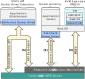
\includegraphics{software-architecture}
    \caption[Three different sharing methods are made possible by our framework. The SmartIO driver abstracts away the physical location of a remote resource]
    {The software architecture of SmartIO. Three different sharing methods are made possible by our framework: \textbf{(1)}~\gls{dl}, \textbf{(2)}~\gls{mdev}, and \textbf{(3)}~using the \gls{sisciapiext}. The SmartIO driver, shown as layer \textbf{(B)}, abstracts away the physical location of remote resources, for both the shared device and software using the device.}
    \label{fig:architecture}
\end{figure}


In this section we address the challenges of \cref{sec:challenges}, and give a bottom-up summary of the implementation of SmartIO.
%
\cref{fig:architecture} illustrates the different components of our framework, and how they fit together.
%
The full implementation details can be found in the published papers, with \cref{paper:tocs} providing a detailed description of the entire solution as a whole.



\subsection{Low-level NTB driver}\label{sec:ntb-driver}
SmartIO is implemented on top of the \gls{ntb} interconnection solution from Dolphin.
%
The low-level \gls{ntb} driver, illustrated as layer \textbf{(A)} in \cref{fig:architecture}, provides the fundamental \gls{pcie} networking infrastructure and memory mapping functionality which SmartIO builds on.
%
Individual systems may contribute parts, or \emph{\glspl{segment}}, of their local memory to a distributed, shared memory space. 
%
\Glspl{memorysegment} in remote machines may be mapped into the local address space of a system by using the \gls{ntb}, as explained in \cref{sec:idea}.
%
Moreover, \gls{userspace} applications may use the \gls{sisciapi} to interact with the \gls{ntb} driver to manage \glspl{memorysegment} and implement shared-memory communication.



\subsection{SmartIO driver}\label{sec:smartio-driver}
The SmartIO driver, shown as layer \textbf{(B)} in \cref{fig:architecture}, runs on all machines in the cluster.
%
It acts as an abstraction layer, providing a logical decoupling of devices and which physical machines they are installed in (\glspl{lender}).
%
Neither devices nor software need to consider where resources physically reside, since SmartIO resolves this on behalf of both devices and a machines using them (\glspl{borrower}).
%
By providing this abstraction, the SmartIO driver is the first step towards \gls{dl}, \gls{mdev}, and the \gls{sisciapiext}, presented in \cref{sec:lending,sec:mdev,sec:api} respectively.


Devices registered with SmartIO are assigned a unique identifier which allows machines to refer to a device without needing to specify the \gls{lendermachine}.
%
Internally, the SmartIO driver keeps track of devices and \glspl{lender}, and uses this device identifier to look up machines, devices, and which \gls{ntb} to use.
%
The SmartIO driver is also responsible for making \glspl{devicebar} available as \glspl{sharedsegment}, making it possible for \glspl{borrowermachine} to memory map remote device memory into their local address space (\gls{mmio}).



Most important is the SmartIO driver's responsibility of mapping \glspl{memorysegment} \textbf{on behalf of a device} and returning the \gls{io} addresses to these maps, \textbf{as seen by the device}.
%
The SmartIO driver works out the physical locations of devices and \glspl{memorysegment},~i.e., which machines they reside in and which \glspl{ntb} a device must use in order to reach a \gls{segment}.
%
Note that a \gls{segment} can reside in memory of the machine using the device~(the \gls{borrower}), in memory of the machine where the device is installed~(the \gls{lender}), or a different cluster machine altogether.
%
A segment can even be allocated in device memory of another device, as the SmartIO driver can assist in mapping device \glspl{bar} and enabling \gls{p2p} between devices.
%
\Glspl{borrower} are not required to know anything about the \emph{device-side} \gls{io} addresses returned by our SmartIO driver, other than the fact that they resolve to the same address space as the device.
%
This allows both a \gls{borrower} and the device to remain agnostic about the underlying, physical \gls{pcie} topology, as they can rely on the SmartIO driver to resolve paths in the cluster network and map resources through the appropriate \glspl{ntb}.



The SmartIO driver solves the challenge of managing multiple address spaces, as described in \cref{sec:challenges}.
%
For example, a \gls{borrower} can request a \gls{memorysegment} in a different machine is mapped so that the device may use \gls{dma} to it.
%
Our SmartIO driver will look up which machine the \gls{memorysegment} is in, look up the \gls{lendermachine} and which (device-side) \gls{ntb} it must use, configure the \gls{ntb}, map the \gls{memorysegment} for the device, and return the device-side \gls{io} address of this map back to the \gls{borrower}.
%
The \gls{borrower} can then use this \gls{io} address when interacting with the device in order to initiate the \gls{dma} transfer, and the device is able to reach the \gls{memorysegment} through the lender's \gls{ntb}.
%
\Glspl{borrower} do not need to be aware of the internal \gls{io} address space layout of a \gls{lender}.
%
As it happens, \glspl{borrower} do not even need to know which physical machine the \gls{lender} is.



With the abstraction the SmartIO driver provides, our framework is able to facilitate the sharing and use of remote resources (both memory and devices) as described in \cref{sec:lending,sec:mdev,sec:api}.
%
More details on how SmartIO resolves the paths between devices and other memory resources that must be mapped (for devices) are given in the papers, particularly in \paperref{tocs}.
%
However, please note that the SmartIO driver is not mentioned explicitly by name in the papers, as it is the unifying base for the sharing methods.
%
Instead, the description of its functionality is interleaved with the implementation details of these methods.



\subsection{Device Lending}\label{sec:lending}
\Gls{dl}, illustrated as arrow \textbf{(1)} in \cref{fig:architecture}, makes it possible to share and distribute devices to remote \glspl{hostmachine}.
%
The devices become part of the system they are shared with, allowing application software, device drivers, and even the \gls{os} to use them as if they were locally installed.
%
While \gls{dl} only allows individual \glspl{devicefunction} to be distributed to a single machine at the time, it is nevertheless highly suitable in the case where a device has a complex or proprietary device driver as no modifications to existing software is required.


As mentioned in \cref{sec:idea}, it is possible to map the device memory regions, or \glspl{bar}, of a remote device through an \gls{ntb}.
%
Using the \gls{ntb}, a local \gls{cpu} can perform memory operations on a remote device, such as reading from and writing to device registers.
%
Conversely, local resources, such as \gls{ram} and interrupt addresses, can in turn be mapped for the remote device itself. 
%
This allows the remote device to use \gls{dma} through the \gls{ntb} and trigger interrupt routines on the local \gls{cpu}.
%
The SmartIO driver, as explained in \cref{sec:smartio-driver}, eliminates the complexity of managing multiple address spaces: a user may rely on the SmartIO driver to map resources through the appropriate \glspl{ntb} and provide \gls{io} addresses corresponding to a device's address space.
%
However, as pointed out in \cref{sec:challenges}, we still need to make sure that device drivers use this functionality without requiring that they be re-written. 
%
More precisely, we need a mechanism for \emph{transparently} injecting resolved \gls{io} addresses, without the devices or their drivers being aware of this.



\begin{figure}
    \centering
    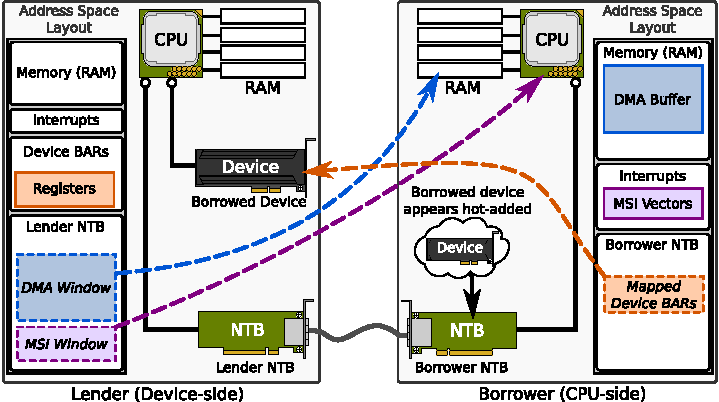
\includegraphics[width=.99\textwidth]{device-lending}
    \caption
    [The memory regions of a remote device is mapped for the \glsfmtshort{cpu} on the borrower, so that it can read and write to device registers. Local resources are mapped for the device, so that it may use \glsfmtshort{dma} and trigger interrupts. \Glsentrytext{dl} inserts a \glsentrytext{shadowdev} into the local device tree using these mappings, making remote device access transparent to both \glsfmtshort{cpu} and device.]
    {The memory regions of a remote device is mapped for the \gls{cpu} on the borrower, so that it can read and write to device registers. Local resources are mapped for the device, so that it may use \gls{dma} and trigger interrupts. \Gls{dl} inserts a \gls{shadowdev} into the local device tree using these mappings, making remote device access transparent to both \gls{cpu} and device.}
    \label{fig:device-lending}
\end{figure}


\Gls{dl} solves this by inserting a ``\gls{shadowdev}'' into the local \gls{pcie} device tree on the \gls{borrower}, as depicted in \cref{fig:device-lending}. 
%
The \gls{shadowdev} makes it appear as if the remote device has been \gls{hotadded} to the local system, and provides us with a mechanism for intercepting interactions with the device by the \gls{os} and any device drivers. 
%
We make sure that a device driver attempting to memory map the device's \glspl{bar} use addresses that map through the \gls{ntb}, without the driver being aware that the device is actually remote.
%
Similarly, when the device driver configures interrupts, we are able to intercept this and inject an address that map through the \gls{lender}'s \gls{ntb}, again without the driver being aware.



\begin{figure}
    \centering
    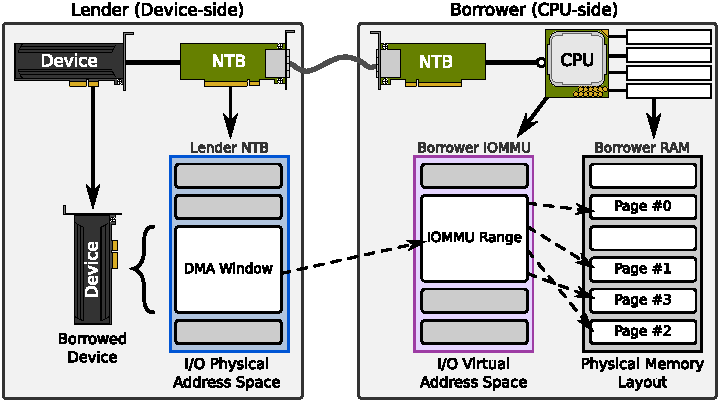
\includegraphics[width=.99\textwidth]{dma-window}
    \caption[The borrower's \glsfmtshort{iommu} is used to create a single continuous memory range that may be mapped through the lender's \glsfmtshort{ntb} in advance. Adding and removing memory pages from the local \glsfmtshort{iommu} domain is inexpensive compared to actively communicating with the remote lender~machine]
    {The \gls{borrower}'s \gls{iommu} is used to create a single continuous memory range that may be mapped through the \gls{lender}'s \gls{ntb} in advance. Adding and removing memory pages from the local \gls{iommu} domain is inexpensive compared to actively communicating with the remote \gls{lendermachine}.}
    \label{fig:dma-window}
\end{figure}


The \gls{shadowdev} also provides us with the means to detect when a device driver is allocating \gls{dma} buffers and making memory available for \gls{dma} transfers.
%
Unlike \glspl{devicebar} and \gls{msi} addresses, memory addresses for \gls{dma} buffers are not known in advance, as mentioned in \cref{sec:challenges}.
%
Mapping \glspl{bar} and interrupts is a one-time operation.
%
The pages used for \gls{dma} memory buffers, however, may be scattered in physical memory.
%
A driver may even initiate several transfers to different parts of memory altogether.
%
Mapping individual memory pages through the \gls{lender}'s \gls{ntb} would not only exhaust the number of available entries in its \gls{lut}, but communicating with the \gls{lendermachine} in order to map these pages dynamically would introduce communication latency in the critical performance path.



To solve this, \gls{dl} relies on the \gls{iommu} on the \gls{borrower}, as depicted in \cref{fig:dma-window}.
%
We can prepare a continuous memory address range \emph{in advance} using the \gls{borrower}'s \gls{iommu}.
%
This range can be mapped through the \gls{lender}'s \gls{ntb} with a single map, or ``\gls{dmawindow}'', even before any device drivers are using the device.
%
When a device driver, at a later point, allocates \gls{dma} buffers, we can simply add these addresses to the \gls{iommu} range.
%
This way, we can avoid making any assumptions about the memory used by a device driver.
%
Additionally, since this is an entirely local operation (on the \gls{borrower}), communication with the remote \gls{lendermachine} is avoided.
%
All address translations between the different address domains are done in \gls{ntb} and \gls{iommu} hardware, ensuring that this solution is able to achieve native \gls{pcie} performance in the data path.



A more technical description of the implementation of \gls{dl} can be found in \paperref{tocs:lending}, including details about the \gls{shadowdev} and \glspl{cfgcycle}.
%
\paperref{tocs:lending-p2p,cc:p2p} explain how \gls{dl} is able to support \gls{p2p} \gls{dma} between multiple borrowed devices, even when they reside in different \glspl{lendermachine}.
%
In addition, \paperref{tocs:lending-dma,tocs:disc-devs} explain how we can use the \emph{\gls{lender}'s} \gls{iommu} to remap \glspl{dmawindow} from high to low memory addresses for devices with addressing limitations.



\subsection{MDEV}\label{sec:mdev}
Our \gls{mdev} implementation, shown as arrow \textbf{(2)} in \cref{fig:architecture}, enables the Linux~\gls{kvm} to \emph{\lgls{passthrough}{pass through}} borrowed devices to \glspl{vm}.
%
This \gls{passthrough} allows software running in a \gls{vmguest} to use the physical device directly, without compromising the memory isolation provided by the virtualization.
%
Whereas \gls{dl} is only supported for machines running Linux, \gls{mdev} makes it possible to share devices with \emph{any} \gls{guestos} (running in the \gls{vm}).
%
Using \gls{mdev}, devices are no longer tightly coupled with the \glspl{hostmachine} they are installed in, allowing \glspl{vm} to be distributed across different \glspl{host} in the cluster while benefiting from the bare-metal performance of direct access to physical hardware.


\begin{figure}
    \centering
    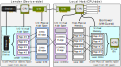
\includegraphics[width=.99\textwidth]{mdev-dma}
    \caption
    [The \glsfmtshortpl{iommu} on both sides of the \glsfmtshort{ntb} must be used in order to pass through a remote device to a local \glsfmtshort{vm}. The borrower's \glsfmtshort{iommu} is used to provide continuous memory ranges for scattered \glsfmtshort{vm} memory, while the lenders's \glsfmtshort{iommu} is used to mirror the guest-physical layout for the device]
    {The \glspl{iommu} on both sides of the \gls{ntb} must be used in order to \lgls{passthrough}{pass through} a remote device to a local \gls{vm}. The \gls{borrower}'s \gls{iommu} is used to provide continuous memory ranges for scattered \gls{vm} memory, while the \gls{lender}'s \gls{iommu} is used to mirror the \gls{guestphys} layout for the device.}
    \label{fig:mdev-dma}
\end{figure}


Our \gls{mdev} sharing method is implemented using the mediated device driver \gls{paravirtualization} interface~\cite{url:LinuxMDEV}.
%
Comparable to the \gls{shadowdev} used by \gls{dl}~(\cref{sec:lending}), this interface makes it possible to \gls{trap}~(handle) certain operations, such as \glspl{cfgcycle} and device resets, and to set the memory addresses of the device's \glspl{bar}.
%
However, unlike \gls{dl}, we do not have any means of controlling which \gls{io} addresses a device driver should use when initiating \gls{dma} transfers.
%
In \gls{dl}, we create a single, continuous \gls{iommu} range ahead of time, and map it through the \gls{lender}'s \gls{ntb}. 
%
We are able to detect when a device driver is preparing \gls{dma} buffers through the \gls{shadowdev}, and can inject the prepared device-side \gls{io} address of our \gls{dmawindow}.
%
In contrast, a device driver running in the \gls{vmguest} is completely isolated, leaving us without any equivalent mechanism to inject \gls{io} addresses we can control.
%
The only possible option is to make sure that the device is mapped to the same virtual address space as the \gls{vm}, as pointed out in \cref{sec:challenges}.



In order for a device to \gls{dma} to \gls{vm} memory, the \gls{hostphys} memory pages backing the emulated memory needs to be locked in physical \gls{ram}.
%
In practice, all memory allocated for a \gls{vmguest} must be mapped for the device, as a device driver or application running in the \gls{guest} may try to use any \gls{guestphys} address when interacting with the device.
%
However, as this is handled by the \gls{hypervisor} for normal \gls{passthrough} of a local device, the mediated device driver interface does not provide any notification of when this memory is allocated by a \gls{vmemulator}.
%
As such, we have no reliable method of detecting \gls{hostphys} memory that needs to be mapped. %through the \gls{ntb}.
%
To further complicate matters, we can not rely on modifying existing \gls{emulator} software to solve this issue, as per our objectives stated in \cref{sec:problem}.
%
Nevertheless, it is possible to rely on an assumption:
%
before a device can use \gls{dma}, it must be enabled in its \gls{cfgspace}.\footnote{Enabling the ``Bus Master'' bit in the command register enables \gls{dma} for a device.}
%
Since the mediated device driver interface makes it possible to \gls{trap} \glspl{cfgcycle}, our \gls{mdev} implementation waits for \gls{dma} to be enabled.
%
By then, the \gls{emulator} has allocated all of the \gls{host}~memory it needs for the \gls{vm}, and we are able to use the \gls{hypervisor} to lock the \gls{hostphys} pages of the \gls{vm} in physical \gls{ram} and resolve their physical addresses.



With the \gls{hostphys} memory backing the \gls{vm} resolved, we can now map it for the device.
%
However, when \lgls{passthrough}{passing through} a local device, the \gls{hypervisor} places the device in a \gls{iommu} domain with \gls{io} virtual addresses that correspond to the \gls{vm}'s address layout.
%
In our case, the device resides in a \emph{different} machine,~i.e., the \gls{lender}.
%
Additionally, the \gls{hostphys} memory pages used by the \gls{emulator} may be scattered throughout physical \gls{ram}.
%
Our \gls{mdev} implementation solves this by using both the \gls{iommu} on the \gls{borrower} and on the \gls{lender}, as shown in \cref{fig:mdev-dma}.
%
The \gls{borrower}'s \gls{iommu} is used to provide continuous address ranges that can be mapped through the \gls{lender}'s \gls{ntb}, or \glspl{dmawindow}.
%
The \gls{iommu} on the \gls{lender} is used to map the device to a virtual \gls{io} address space that mirrors the \gls{vmguest}'s, allowing a device driver running in the \gls{vmguest} to initiate \gls{dma} transfers using \gls{guestphys} addresses.



\paperref{tocs:mdev} provides more information about the \gls{mdev} implementation, including a more detailed description of the mediated device driver interface and the functionality it provides. 
%
In the same section, we also explain a workaround for interrupts, by relaying them from the \gls{lender} to the \gls{borrower}.
%
Finally, a method of probing the \gls{kvm} using well-defined starting addresses for high and low memory is outlined, in order to pinpoint the \gls{guestphys} memory layout and conserving \gls{ntb} maps.



\subsection{API extension}\label{sec:api}
As mentioned in \cref{sec:ntb-driver}, a \gls{userspace} application may memory-map \glspl{sharedsegment} into its own local address space using the \gls{sisciapi}.
%
Application processes running on different machines may read and write to remote memory, as if it was reading or writing to local \gls{ram}.
%
Our \gls{apiext}, depicted as arrow \textbf{(3)} in \cref{fig:architecture}, adds device-oriented programming semantics and device driver support functionality to this shared-memory \gls{api}.
%
This extension makes the core SmartIO capabilities, as described in \cref{sec:smartio-driver}, available through the same shared-memory \gls{api} used to write cluster applications.



The \glspl{bar} of a device is exported as \glspl{sharedsegment} that may be mapped by the application, providing access to device registers and other device memory (\gls{mmio}).
%
Several application processes running on different machines may even access such memory mapped \glspl{bar} at the same time.
%
Similarly, \glspl{memorysegment} can be mapped for a device (as \glspl{dmawindow}), allowing devices to use native \gls{dma} to access \gls{sharedsegment} directly.
%
These \glspl{segment} can reside in local \gls{ram} of the \gls{lender}, the \gls{borrower}, or a different cluster machine entirely.
%
\Glspl{segment} can even be allocated in device memory of \emph{other} devices.
%
SmartIO dynamically resolves the location of \glspl{segment} and devices in the cluster network, and can set up and tear down the necessary \gls{ntb} maps for the respective machines.
%
The \gls{apiext} also provides functionality for allocating \glspl{segment} associated with a device, and using access pattern hints in order for SmartIO to determine which machine it should allocate memory in.



By allowing device drivers to be implemented as part of the application software, we make it possible for devices and device operation to become part of the same shared global address space as distributed shared-memory applications.
%
Thus, device drivers can be implemented in a way that fully utilize the capabilities of \gls{pcie} networks.
%
For instance, applications may stream data to several destinations in a single operation, replicating data across several machines by relying \gls{multicasting} support in \gls{pcie} hardware.
%
A programmer can exploit memory locality to optimize data flow through the network without needing to be aware of the actual network topology, by specifying memory access pattern hints and allowing SmartIO to decide where \glspl{segment} should be allocated.
%
It is even possible to combine the \gls{apiext} with the other sharing methods of SmartIO, allowing \gls{disaggregation} of \emph{borrowed} resources.
%
An example of this is would be a machine using \gls{dl} to borrow a remote \gls{gpu} capable of \gls{gpudirect}~\cite{url:GPUDirect,url:Rosetti2014}, allowing the device to be operated by the native driver, and then using the \gls{apiext} to export \gls{gpu} memory as a \gls{sharedsegment}.
%
Application processes on other machines can then memory map this (remote) device memory \gls{segment}, allowing them to read and write directly to it as if it was local memory.



Since the \gls{apiext} is built on the underlying SmartIO driver, software can be written in a way that does not need to consider whether resources are local or remote.
%
However, using the \gls{apiext} requires the implementation of new device driver software.
%
Implementing a driver from scratch may not be a viable option in many cases, as it typically entails a considerable engineering effort.
%
After all, the strength of \gls{dl} and the \gls{mdev} implementation is precisely that they do not require any modifications to existing device driver software.
%
Even so, being able to integrate device drivers into the cluster application itself may potentially be very useful for some application domains.
%
The possibilities created by the \gls{apiext} are perhaps best exemplified by our proof-of-concept \gls{nvme} driver, described in \cref{sec:nvme-driver}.
%
This driver shows how a non-\gls{sriov} \gls{nvme} can be \gls{disaggregated} in software and shared by several machines, as well as how we can use the \gls{apiext} for \gls{disaggregating} memory resources.
%
A more specific description of the functionality added to \gls{sisci} by our \gls{apiext} can be found in \paperref{tocs:api}.



\subsection{Proof-of-concept NVMe driver}\label{sec:nvme-driver}
Most device drivers are written in a way that assumes exclusive control over the device.
%
In most cases, a device can only be distributed to a single \gls{borrowermachine} at the time, preventing others from using it while it is used.
%
Some devices implement \gls{sriov}~\cite{spec:SRIOV}, making a single physical device to appear as multiple (virtual) device functions, or \glspl{vf}.
%
Using \gls{dl} or our \gls{mdev} implementation, it is possible to distribute such \glspl{vf} to \glspl{borrower}.
%
However, due to the complexity of supporting virtualization in hardware, \gls{sriov} is not widely available, especially not for commodity devices.
%
By facilitating \gls{disaggregation} in \emph{software} instead, our \gls{sisciapiext}~(\cref{sec:api}) makes it possible for several application processes running on different machines to share the same device (\gls{function}).
%
As a demonstration of this software-enabled \gls{disaggregation}, we have implemented an \gls{nvme} driver as a \gls{userspace} \gls{sisci} application.
%
\Glspl{nvme} are highly parallel by design, and the interaction between driver software and \gls{nvme} hardware is standardized~\cite{spec:NVMe}, making it possible to implement a general device driver for them.


\begin{figure}
    \centering
    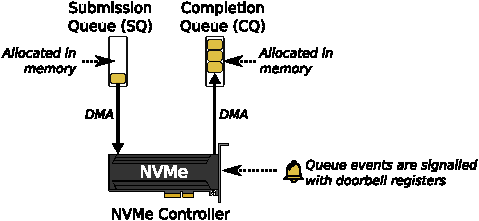
\includegraphics{nvme}
    \caption
    [\Glsfmtshortpl{nvme} support parallel and asynchronous operation by using independent queues. Queues are hosted in memory, and an \glsfmtshort{nvme} uses \glsfmtshort{dma} to fetch commands]
    {\Glspl{nvme} support parallel and asynchronous operation by using independent queues for submitting \gls{io} commands and receiving completions. Queues are hosted in memory, and an \gls{nvme} uses \gls{dma} to fetch commands and post completions.}
    \label{fig:nvme}
\end{figure}



\Cref{fig:nvme} shows how \glspl{nvme} support asynchronous operation by using a system of paired command \glspl{sq} and \glspl{cq}.
%
Both types of queues are data structures that are allocated in memory by discretion of the driver, and may be placed in \emph{any} memory location.
%
The driver submits \gls{io} commands, such as reading or writing $N$ blocks from storage, to an \gls{sq}.
%
The \gls{nvme} will use \gls{dma} to fetch commands from the \gls{sq}, and once a command is carried out, the \gls{nvme} posts the command completion status to the associated \gls{cq} (also using \gls{dma}) containing the status of the command.
%
``\Glspl{db}'' on the \gls{nvme} device are used to signal when new commands should be fetched, and each queue has its own \gls{db}.
%
Furthermore, as \emph{multiple} of these queue pairs can be created, \glspl{nvme} avoid any contention in the command submission and completion paths.
%
An example of this is a multi-core \gls{cpu} that assigns an \gls{sq} and an associated \gls{cq} per \gls{cpu} core, allowing each core to operate the \gls{nvme} independent of others.


\begin{figure}
    \centering
    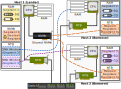
\includegraphics[width=.99\textwidth]{nvme-driver}
    \caption
    [Several machines can operate the same \glsfmtshort{nvme} simultaneously by distributing queues]
    {Several machines can share and operate the same \gls{nvme} simultaneously by distributing queues. Using the \gls{sisciapiext}, \glspl{memorysegment} with the queues' data structures can be mapped for the device, and \glspl{db} can be memory mapped for application processes.}
    \label{fig:nvme-driver}
\end{figure}


As shown in \cref{fig:nvme-driver}, our own driver implementation works by taking this one step further, allowing \glspl{cpu} in different machines to operate an \gls{nvme} simultaneously using their own queue pairs.
%
Each machine allocates a \gls{memorysegment} where it sets up the queues' data structures, and uses the \gls{apiext} to map these segments for the device as \glspl{dmawindow}.
%
This allows the \gls{nvme} to read \gls{sq} memory and write to \gls{cq} memory the same way it would access local memory, using native \gls{dma}.
%
Likewise, as \glspl{devicebar} are automatically exported by SmartIO as \glspl{segment}, all machines can memory map \glspl{db} for their respective queues.
%
Since queues are completely parallel, all the machines can submit \gls{io} commands and receive completions entirely independent of each other, once the queues are configured.
%
Note that all machines are able to operate the \gls{nvme} at the same time, including the \gls{lender}.
%
The software is the same regardless of which machine it runs on, as SmartIO keeps track of where the \glspl{segment} and the device reside.


\begin{figure}
    \centering
    \begin{subfigure}{\linewidth}
        \centering
        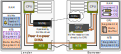
\includegraphics[width=.99\textwidth]{nvme-local-gpu}
        \caption{Storing from and loading into the memory of a \gls{gpu} residing in the \gls{borrower}.}
        \label{fig:nvme-local-gpu}
    \end{subfigure}
    \par\vspace{5mm}
    \begin{subfigure}{\linewidth}
        \centering
        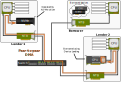
\includegraphics[width=.99\textwidth]{nvme-remote-gpu}
        \caption{Storing from and loading into the memory of a borrowed (remote) \gls{gpu}.}
        \label{fig:nvme-remote-gpu}
    \end{subfigure}
    \caption
    [Our proof-of-concept \glsfmtshort{nvme} driver is able to map \glsfmtshort{gpu} memory for an \glsfmtshort{nvme} using the SmartIO \glsfmttext{apiext}, making it possible to load and store data directly from \glsfmtshort{gpu} memory]
    {By relying on \gls{gpudirect} to expose \gls{gpu} memory through the \gls{gpu}'s \glspl{bar}, our proof-of-concept \gls{nvme} driver is able to map \gls{gpu} memory for an \gls{nvme} using the SmartIO \gls{apiext}. This makes it possible to load and store \gls{gpu} data directly, without unnecessarily copying it via \gls{ram}.}
    \label{fig:nvme-gpu}
\end{figure}


\begin{figure}
    \centering
    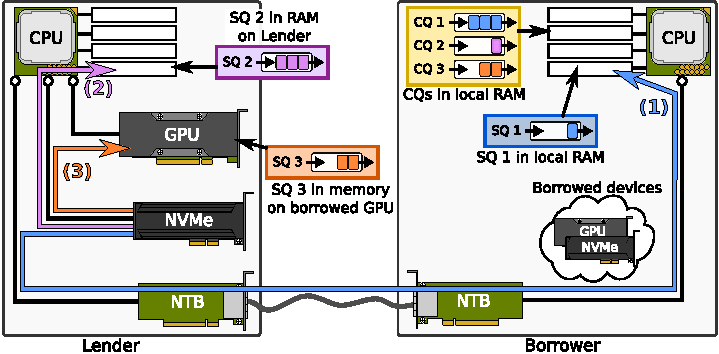
\includegraphics{nvme-queues}
    \caption
    [By using access pattern hinting, it is possible to consider memory locality without requiring the driver implementation to be aware of the underlying \glsfmtshort{pcie} topology]
    {Our \gls{nvme} driver implementation relies on SmartIO to decide where \glspl{segment} containing queues should be allocated. By using access pattern hinting, it is possible to consider memory locality without requiring the driver implementation to be aware of the underlying \gls{pcie} topology.}
    \label{fig:nvme-queues}
\end{figure}


As mentioned in \cref{sec:api}, while using \gls{apiext} requires developing a new device driver, such as our proof-of-concept \gls{nvme} driver, the benefit is that device operation can become part of the cluster application itself.
%
Because SmartIO abstracts away the location of devices and \glspl{memorysegment}, the complexity of developing such distributed drivers is somewhat alleviated as software can be written in a way that does not need to consider whether resources are local or remote.
%
Any memory resource can be mapped for the device, regardless of its location in the cluster.
%
An implementation can exploit this in order to optimize the movement of data through the network---without needing to consider the actual \gls{pcie} topology.
%
It is even possible to combine the use of the \gls{apiext} with the other sharing methods of SmartIO.
%
Our \gls{nvme} driver demonstrates some of the possibilities created by the \gls{apiext}: 
%
\begin{description}
    \item[Remote \gls{gpu} access] (\cref{fig:nvme-gpu}):
        %
        Many \gls{gpu}-accelerated applications, such as big~data and machine~learning tasks, require access to data on a storage device.
        %
        Traditionally, loading data from a storage device and into \gls{gpu} memory involves first reading data to system memory, and then copy it onto the \gls{gpu}.
        %
        Likewise, storing the result of a \gls{gpu} computation involves copying it out of the \gls{gpu} to system memory, and then writing it to storage.
        %
        Since datasets used in typical big~data and machine~learning tasks can be as large as hundreds of terrabytes, \gls{gpu} applications become bounded by transfers between storage and \gls{gpu}.
        %
        To overcome this, some \glspl{gpu} support \gls{p2pdma}, making it possible to load data directly into \gls{gpu} memory and avoid unnecessary copies via system memory~\cite{Bergman2019,url:Thompson2019}.
        %
        For Nvidia \glspl{gpu}, this functionality is supported through the \gls{gpudirect}~\gls{api}~\cite{url:GPUDirect}, which makes on-board \gls{gpu} memory accessible through the \gls{gpu}'s \glspl{bar}.
        %
        As explained in \cref{sec:smartio-driver}, SmartIO automatically exports \glspl{devicebar} as \glspl{memorysegment}, which can be mapped for a device using the \gls{apiext}.
        %
        Our proof-of-concept \gls{nvme} driver use this to enable an \gls{nvme} to read and write directly to the memory of both local \glspl{gpu} and \emph{borrowed} \glspl{gpu} (using \gls{dl}), as seen in \cref{fig:nvme-local-gpu,fig:nvme-remote-gpu} respectively.
        %
        Note that the \gls{gpu} is operated by the native \gls{gpu} driver in both scenarios, but we still use the \gls{apiext} to disaggregate its device memory.

    \item[Memory locality optimizations] (\cref{fig:nvme-queues}):
        %
        In \gls{pcie}, the latency of transactions are affected by the number of switch chips they need to traverse.
        %
        Particularly memory reads are affected; the longer the path between a device and the memory it reads from, the higher the latency becomes, as \gls{pcie} transactions have to travel further.
        %
        As described in \cref{sec:api}, a programmer can rely on the \gls{apiext} to decide where \glspl{segment} should be allocated, based on memory access pattern hinting.
        %
        In the case of our \gls{nvme} driver, we can use this functionality when creating \glspl{segment} for queue memory, as illustrated in \cref{fig:nvme-queues}.
        %
        By specifying that the \gls{segment} containing \glspl{cq} will be written to by the \gls{nvme}, and read by the \gls{borrower}'s \gls{cpu}, SmartIO will decide to allocate the \gls{segment} in memory closer to the \gls{cpu},~i.e., in the \gls{borrower}'s local \gls{ram}.
        %
        Similarly, a segment with an \gls{sq} can be allocated in the \gls{lender}'s \gls{ram} by specifying that the \gls{nvme} will read from it and the \gls{cpu} will only write to it, shown as SQ1 in \cref{fig:nvme-queues}.
        %
        It is even possible to use memory of \emph{another device} for \glspl{sq}.
        %
        By mapping \gls{gpu} memory for the device, as explained above, it is possible to allocate the \gls{sq} on a borrowed \gls{gpu} that is close to the \gls{nvme}, depicted as SQ2 in \cref{fig:nvme-queues}.

\end{description}


A more technical description of the implementation of the proof-of-concept \gls{nvme} driver can be found in \paperref{tocs:nvme}.
%
Here, we describe how the driver is split into a manager and a client component, with the manager being responsible for resetting the device and assigning queues to clients.
%
We also explain how our implementation can support multi-path fail-over, and how \gls{pciemulticasting} can be used to replicate data loaded from storage across machines in a single operation.
%
Details on how it is possible to run the \gls{nvme} driver as part of a \gls{cuda} kernel can also be found here, making it possible for software running on the \gls{gpu} to control an \gls{nvme} entirely without any involvement of the \gls{cpu}.



\section{Performance measurements}\label{sec:eval}
Some selected performance graphs here, demonstrating zero-overhead :)



\section{Related work}\label{sec:rw}
As a complete solution, SmartIO encompasses multiple components that each could potentially be discussed at great length in order to place them in proper context.
%
However, at its core, SmartIO is a framework for sharing \gls{io} resources and facilitating remote access.


In an attempt to condense related work down to the most relevant, we broadly divide it

%many solutions already exist

Broadly divided into the following categories:
\begin{itemize}
    \item PCIe-based solutions
    \item memory disaggregation
    \item shared-memory
    \item ladon
    \item 
\end{itemize}
%\subsection{RDMA-based solutions}

%\subsection{PCIe-based solutions}
\begin{itemize}
    \item rdma stuff
    \item fabric partitioning: mr-iov, broadcom/microsemi chips with partitioning
    \item ladon (and other ntb stuff)
    \item disaggregation
\end{itemize}


	\chapter{Conclusion}\label{chapter:conclusion}
As distributed and parallel computing applications are becoming increasingly compute-intensive and data-driven, \gls{io} performance demands are ever growing.
%
Computing accelerators (such as \glspl{fpga} and \glspl{gpu}), high-throughput \glspl{nic}, and fast storage devices like \glspl{nvme}, are now commonplace in most modern computer systems.
%
Nevertheless, distributing such \gls{io} resources in a way that maximizes both performance and resource utilization is a challenge for heterogeneous computing clusters. 
%
To avoid that individual machines becoming performance bottlenecks, resources must be shared efficiently between machines in the cluster.



In this dissertation, we have addressed this challenge and presented our SmartIO framework for sharing \gls{io} resources between machines connected over \gls{pcie}.
%
Our SmartIO framework effectively makes all machines, including their internal devices and memory, part of a common \gls{pcie} domain.
%
Resources in remote machines can be used as if they were installed locally, without any performance degradation compared to local access and without requiring adaptions to device drivers or application software.
%
The hard separation between local and remote is blurred out, as machines can freely share their internal devices and memory resources with other machines in the cluster. 



\section{Summary}\label{sec:summary}
% - What was the target problem?
Connecting two or more computer systems over \gls{pcie} is possible by using \glspl{pcientb}.
%
\Glspl{ntb} have memory address translation capabilities that makes it possible for a machine to map \glspl{segment} of remote memory directly into local address space.
%
However, leveraging \glspl{ntb} to share the internal devices and memory of a machine with other, remote machines is a challenge, as the use of a remote resource requires software to be aware of the fact that the resource is on the other side of an \gls{ntb}.
%
For example, a device driver operating a remote device must use addresses that correspond to the remote device's address space when initiating \gls{dma} transfers or configuring interrupts.
%
This additional complexity makes it infeasible to rely on \glspl{ntb} alone to implement a resource sharing solution, as it would require extensive modifications to existing software.



% - What did you develop?
To solve this, we have developed our SmartIO framework for sharing devices and memory resources between machines connected with \glspl{ntb}.
%
Our solution consists of ``\glspl{lender}'', machines lending out one or more of its internal devices, and ``\glspl{borrower}'', machines using such a device.
%
Machines can act as \gls{lender} and \gls{borrower} at the same time, making SmartIO fully distributed.
%
Any type of \gls{pcie} device may be shared, as SmartIO is built on standard \gls{pcie}.
%
SmartIO keeps track of which machines devices and \glspl{memorysegment} reside in, and is able to map resources on behalf of devices and resolve memory addresses as they are seen by devices.
%
As such, SmartIO provides a logical decoupling of devices and which \glspl{lendermachine} they are installed in, solving the challenge of managing multiple address spaces and making remote resources appear and behave as if they are local.




SmartIO supports three different methods of device sharing:
%
\begin{itemize}
    \item Our \textbf{\gls{dl}} sharing method makes it possible to dynamically assign a \gls{pcie} device to a remote \gls{borrowermachine}.
        %
        By using a ``\gls{shadowdev}'', the device appears \gls{hotadded} to the local device tree on the \gls{borrower}.
        %
        The fact that the device is remote is made transparent to the system, allowing the device to be used by native device drivers and application software as if it was locally installed.


    \item Our \textbf{\gls{mdev}} extension to the \gls{kvm} makes it possible to distribute devices to \glspl{vm} running on remote machines, by facilitating \emph{\gls{passthrough}} of a device to the \gls{vmguest}.
        %
        Application software and device drivers running inside the \gls{vmguest} can directly interact the physical device, without compromising the isolation of the virtualized environment.


    \item Our \textbf{\gls{sisciapiext}} makes it possible to \gls{disaggregate} devices and memory resources in software.
        %
        We have extended the \gls{sisciapi} with device-oriented programming semantics and device driver support functionality, making core SmartIO capabilities available through the same shared-memory \gls{api} used to write cluster applications.
        %
        Using this \gls{apiext}, we have also implemented a \textbf{proof-of-concept \gls{nvme} driver} that demonstrates how devices can be \gls{disaggregated} and shared with multiple machines at the same time.
        
\end{itemize}




% - What were the results?
We have performed an extensive performance evaluation, consisting of a comprehensive collection of synthetic performance benchmarking and realistic workloads.
%
We have made a point out of using standard benchmarking software and device drivers, as well as a wide variety of \gls{pcie} devices, in order to demonstrate the completeness of our SmartIO framework.
%
Particularly, we have performed comparison tests where we compare the performance of a workload using remote resources to the same workload running only on a local system.
%
The results prove that, when conditions are similar, the SmartIO sharing methods \textbf{do not add \emph{any} performance overhead} compared to using local resources.
%
Furthermore, we have also explored how different network topologies affect the performance, and have identified situations where the \gls{iommu} can become a potential performance bottleneck.
%
Finally, our exhaustive performance test suite also includes tests using our proof-of-concept \gls{nvme} driver that highlights possibilities that are enabled by our shared-memory approach to device sharing.






\section{Revisiting the problem statement}\label{sec:discussion}
%Although many \gls{disaggregation} solutions for sharing resources over a network already exist, these solutions are often inadequate as discussed in \cref{sec:rw}. 
%%%
%For instance, \gls{disaggregation} solutions based on \gls{rdma} introduce additional software complexity and indirections that lead to a disparity in performance, compared to a local machine using local resources. 
%%%
%\Gls{pcie}-based \gls{disaggregation} solutions do not have such performance issues, since they facilitate the use of resources using native \gls{pcie}.
%%%
%However, \gls{pcie}-based \gls{disaggregation} solutions are limited to sharing devices installed in dedicated servers, as they lack the shared-memory capabilities necessary for sharing the \emph{inner} resources of individual machines. 
%
%
%
%Thus, 
The main goal of this dissertation was not simply to implement yet another \gls{disaggregation} solution, but developing a new, more flexible solution with zero overhead by taking a novel approach:
%
leveraging the memory mapping capabilities of \glspl{ntb} to unify traditional device \gls{io} with distributed, shared-memory computing.
%
Such a solution should allow the inner devices and memory of machines to be shared with, and used by, remote machines in a cluster, as if these resources were local to the remote machines using them.
%
In \cref{sec:problem}, we broke down the challenges of this goal into \crefrange*{obj:distributed}{obj:experiments}:



% How did we answer objectives 1-6? 
% For each objective, state clearly how it was solved and the contribution of it (refer back to contributions in 1.5)
% Also make it clear how the contribution helps solve the overall research question as well.



\objdistributed*%
%
%Using SmartIO, machines act as ``\emph{\glspl{lender}}'' and ``\emph{\glspl{borrower}}''. 
%
%A \gls{lender} registers one or more of its devices with SmartIO, allowing these devices to be used by remote machines.
%%
%A \gls{borrower} is a system or software process that is currently using such a device.
%
SmartIO is fully distributed, allowing \emph{any} machine in the cluster to act as a ``\emph{\gls{lender}}'' or a ``\emph{\gls{borrower}}'', or even acting as both at the same time.
%
Any \gls{pcie} device may be registered with SmartIO and shared, as demonstrated by our comprehensive performance evaluation in \cref{tocs}.
%
As such, we enable a peer-to-peer sharing model, where all machines in the cluster can participate in the sharing through contributing their own resources and using resources shared by others.


We implemented three different sharing methods for our solution: 
%
\begin{itemize}
    \item The \gls{dl} sharing method, explained in \cref{sec:lending}, makes it possible to distribute devices to remote machines.
        %
        %The initial \gls{dl} is described in \cref{nossdav}. Subsequent improvements, such as supporting borrowing devices from several \glspl{lender}, are detailed in \cref{srmpds,cc,tocs}.
        The initial \gls{dl} method is presented in \cref{nossdav}. Subsequent improvements are presented in \cref{srmpds,cc,tocs}.



    \item The \gls{mdev} extension to the \gls{kvm} makes it possible to distribute devices to \glspl{vm} running on remote machines, as detailed in \cref{sec:mdev}.
        %
        The initial \gls{mdev} method is presented in \cref{srmpds}, and improved versions are presented in \cref{cc,tocs}.
        %
        %The initial \gls{mdev} is described in \cref{srmpds}, and an improved version with a mechanism for discovering \gls{guestphys} memory layout is described in \cref{cc,tocs}.



    \item The \gls{apiext} brings device-oriented programming semantics and device driver support functions to the \gls{sisciapi}.
        %
        Using the \gls{apiext}, \gls{userspace} device drivers can be implemented using the same \gls{api} used to implement shared-memory communication using \glspl{ntb}, as explained in \cref{sec:api}.
        %
        The \gls{apiext} is presented in \cref{tocs}.
\end{itemize}
%
These sharing capabilities set SmartIO apart from existing \gls{pcie}-based \gls{disaggregation} solutions (including Ladon~\cite{Tu2013}), as these solutions are only able to share devices in dedicated servers.
%
Thus, our sharing methods solves \cref*{obj:distributed}.





\objtransparent*%
%
Our three sharing methods address this objective in the following ways:
%
\begin{itemize}
    \item \Gls{dl} inserts a remote device into the local device tree of the \gls{host}~\gls{os} by using a ``\gls{shadowdev}''.
        %
        This allows device drivers, application software, and even the (\gls{host})~\gls{os} itself to use the remote device through \emph{native} \gls{os} interfaces, in the same way they would use a local device.
        %
        No adaptations to existing software is required.
        %
        This is further explained \gls{dl} in \cref{nossdav,srmpds,cc,tocs}.
    


    \item \Gls{mdev} enables \gls{passthrough} of a remote device to a \gls{vm}.
        %
        Software running in the \gls{guest}, including device drivers and the \gls{guest}~\gls{os}, may interact with the physical device directly, without escaping the virtualized environment.
        %
        To the \gls{vmguest}, the device appear as locally installed devices.
        %
        No modifications to \gls{vmemulator} software or \gls{host}~\gls{os} is necessary.
        %
        \Gls{mdev} is described in further detail in \cref{srmpds,cc,tocs}.


    \item Using the \gls{sisciapi}, remote \glspl{memorysegment} are mapped directly into the virtual address space of a local application.
        %
        Our \gls{exttosisciapi} makes it possible to map such \glspl{segment} for \emph{devices} as well.
        %
        This enables native \gls{dma} to remote memory resources, as if both the device and the memory being accessed were both installed in the same, local machine.
        %
        Moreover, using the \gls{apiext}, the physical location of both devices and \glspl{memorysegment} are abstracted away.
        %
        \Gls{userspace} device drivers implemented using our \gls{ext} can be written as if all resources are local, similarly to how a local \gls{userspace} device driver (for a local device) would be implemented.
        %
        The \gls{apiext} is described in \cref{tocs}.
\end{itemize}
%
Whether resources are remote or local is made transparent by SmartIO, as remote devices and memory resources both appear and behave as if they are locally installed.
%
In this regard, SmartIO differs from existing \gls{disaggregation} solutions based on \gls{rdma}.
%
Contrary to these solutions, we do not require interacting with a device driver running on the remote system, thus avoiding any \glspl{middlewareservice} or specialized adaptations to existing software.
%
Scaling out becomes significantly easier, as SmartIO allows remote resources to be used natively instead.
%
Thus, this aspect of SmartIO solves \cref*{obj:transparent}.



\objperformance*%
%
%With SmartIO, remote resources can be mapped using the \gls{ntb} and accessed over standard \gls{pcie}.
%
One of the main challenges for our \gls{dl} and \gls{mdev} sharing methods was that local \gls{ram} must be mapped ahead of time in order to avoid communication overhead in the performance-critical path, yet memory used by a device driver can not be known in advance.
%
To overcome this, our SmartIO implementation supports using the \gls{borrower}'s \gls{iommu} to create continuous memory ranges that can be mapped as ``\glspl{dmawindow}'' through the \gls{lender}'s \glspl{ntb} before use.
%
Memory pages can then be dynamically added and removed from these \gls{iommu} ranges locally on the \gls{borrower}, and communication with a remote system in the critical path is avoided.



Once mapped, remote resources are accessed with native \gls{pcie} performance, as all address translations are done in \gls{ntb} (and \gls{iommu}) hardware.
%
In fact, our evaluation in \cref{tocs} prove that, when conditions are similar, SmartIO allows remote resources to be used \emph{without any performance overhead} compared to using local resources.
%
Nevertheless, using remote resources may lead to a longer distance between resources.
%
As such, there are some caveats that must be considered:
%
\begin{itemize}
    \item Longer \gls{pcie} paths affect \gls{dma} performance, particularly \gls{dma} reads, as we uncovered in \cref{srmpds,cc,tocs}.
        %
        This remains an unsolved challenge for \gls{dl} or \gls{mdev}, as we have no control over the memory allocated by a device driver in these instances.
        %
        Therefore, we recommend considering the length of \gls{pcie} paths when designing the cluster.
        %
        The issue of longer \gls{pcie} paths affects drivers implemented using our \gls{sisciapiext} to a lesser extent;
        %
        by using memory access pattern hinting when allocating \gls{dma} buffers, SmartIO will attempt to minimize the distance a device or a \gls{cpu} needs to read across.
        %
        The performance experiment presented in \cref{sec:eval-nvme} demonstrates this.


    \item Our performance experiments in \cref{srmpds,cc,tocs} also revealed that an \gls{iommu} in the data path can negatively affect \gls{dma} performance, as the \gls{iommu} may split large \gls{pcie} transactions into several, smaller-sized transactions.
        %
        This is especially an issue for our \gls{mdev} sharing method, as SmartIO uses the \gls{lender}'s \gls{iommu} in order to map the device to the same \gls{guestphys} address space as the \gls{vm} the device is \lgls{passthrough}{passed-through} to.
        %
        For \gls{dl}, the use of an \gls{iommu} on the \gls{lender} is optional.
        %
        However, the use of an \gls{iommu} on the \gls{borrower} is necessary (except in a few scenarios where it is possible to map the entire \gls{ram} of the \gls{borrower}). 
        %
        Consequently, this may introduce limitations on scenarios where machines act as both \glspl{lender} and \glspl{borrower}, where maximizing \gls{dma} performance is a requirement.
        %
        In the case where device drivers are implemented using the \gls{apiext}, an \gls{iommu} is entirely optional on \emph{both} the \gls{lender} and the \gls{borrower}.
\end{itemize}
%
By making it possible for remote resources to be accessed over native \gls{pcie}, \cref*{obj:performance} is solved.
%
Improving performance issues involving \glspl{iommu} is a candidate for future work.



\objdynamic*%
%
%\Glspl{lender} may even forcefully reclaim their devices, should it be necessary.
%
%
Using SmartIO, resources may be shared without requiring machines to be rebooted.
%
Devices registered with SmartIO can be borrowed by any machine, at any time, using any of the three sharing methods.
%
For example, a machine may borrow a device using \gls{dl} and at the same time run a \gls{vm} that is borrowing another device using \gls{mdev}.
%
The different sharing methods can also be combined, as demonstrated by the proof-of-concept NVMe driver experiment presented in \cref{sec:eval-nvme}.
%
When the device is no longer needed, it can be returned so it may be used by another \gls{borrower}.
%
Through borrowing and returning devices, systems may scale \gls{io} resources up or down based on current workload demands.



Devices are logically decoupled from the machines they are physically installed in, allowing software to be moved to any machine in the cluster.
%
SmartIO keeps track of both \glspl{memorysegment} and devices, and is able to locate resources in the cluster, without requiring that the user knows anything about the underlying \gls{pcie} topology.
%
The shortest path between devices, \glspl{cpu}, and \glspl{memorysegment} is determined automatically, and SmartIO configures \glspl{ntb} along that path in order to map remote memory resources for \glspl{cpu} and devices.
%
Moreover, SmartIO also supports borrowing devices from multiple \glspl{lender} and enabling \gls{p2pdma} transfers between them, as we explain in \cref{tocs}.
%
\Gls{p2p} can be enabled when borrowing devices using \gls{dl} or \gls{mdev}, which is demonstrated in the various \gls{p2p} experiments presented in \cref{cc,tocs}.
%
\Gls{p2p} is also supported when using the \gls{apiext}, which we demonstrate in the proof-of-concept \gls{nvme} driver experiment (\cref{sec:eval-nvme}).
%
\Cref{nossdav,srmpds,cc,tocs} show how our sharing methods make SmartIO a dynamic and flexible sharing framework, thus solving \cref*{obj:dynamic}.




\objdisaggregation*%
%
SmartIO is able to \gls{disaggregate} multi-function devices, such as devices capable of \gls{sriov}, and distribute individual \glspl{devicefunction} to different \glspl{borrower}.
%
An experiment demonstrating this is presented in \cref{tocs}.
%
Devices that do not support \gls{sriov} may be \gls{disaggregated} in \emph{software} instead, using our \gls{exttosisciapi}.
%
Using the \gls{apiext}, a device be borrowed by several machines simultaneously.
%
Our proof-of-concept \gls{nvme} driver presented in \cref{tocs} demonstrate this, where several \glspl{borrower} share the same (non-\gls{sriov}) \gls{nvme}.
%
In other words, the \gls{apiext} enables ``\gls{mriov} in software''.



%The \gls{apiext} provides functions for borrowing and returning devices, mapping \glspl{devicebar} for the application process, as well as mapping \glspl{sharedsegment} for devices.
%
The \gls{apiext} makes it possible to implement device drivers as part of distributed, shared-memory cluster applications. 
%
Any \gls{memorysegment} anywhere in the cluster can be mapped for devices, so they may access them directly, including \glspl{segment} in local \gls{ram} on the \gls{borrower}, \glspl{segment} in \gls{ram} on the \gls{lender}, and even \glspl{segment} in memory of a different cluster machine altogether.
%
\Glspl{devicebar} are also automatically exported by SmartIO as \glspl{sharedsegment}, allowing device memory to be mapped for the application process or even for \emph{other devices} (thus enabling \gls{p2p}).
%
As such, SmartIO supports \gls{disaggregating} device memory.
%
It is even possible to map \gls{multicasting} \glspl{segment} for a device, allowing a device to stream data to multiple destinations in a single operation.
%
Moreover, SmartIO makes it possible to associate \glspl{memorysegment} with a device (rather than a machine in the cluster), allowing the location of \glspl{memorysegment} to be abstracted away in a similar fashion to devices.
%
Not only does this allow software to be moved to any machine in the cluster, but the implementation of device drivers becomes easier as well as they can be written as if all resources are local.
%
SmartIO is able to optimize memory locations without requiring that the user is aware of the underlying \gls{pcie} network topology.
%
The proof-of-concept \gls{nvme} driver experiment presented in \cref{sec:eval-nvme} demonstrates all of these capabilities, proving that \cref*{obj:disaggregation} is solved.



\objexperiments*%
%
We have performed extensive 

As remote devices, standard device drivers and benchmarking software
For example, CUDA, argue that making use of 


% Refer back to the main research question
% How does this move the world forward?



\section{Future work}\label{sec:fw}
%, particularly implementing support for \gls{ats}~\cite{spec:ATS}, which allows devices (and \gls{pcie} switch chips) to cache resolved \gls{io}~addresses.
%
%However, as \gls{ats} requires support in both devices and \glspl{iommu}, it appears not to be widely adopted, especially for commodity hardware.
%

mention new NVMe kernel space driver here

security / safety

disaggregated memory - new interconnects
%gen z interconnect data center level, cxl -> rack interconnect

iommu in tree structures is a challenge - ats? other solutions?


scaling 

%With SmartIO, the hard separation between local and remote is blurred, as remote resources can be used as if they were locally installed and with native PCIe performance.


%Using the \gls{sisciapi}, application memory can be exported as \glspl{sharedsegment}, and \glspl{segment} in remote machines can be mapped into a local application process' virtual address space.
%By building on these concepts, our \lgls{apiext}{extension} makes it possible for a device driver implementation to use all the memory \gls{disaggregation} capabilities of \gls{sisci}, while also providing functionality for abstracting away the location of memory resources and resolving addresses between different address spaces.
%
%A device driver implemented using our \gls{apiext} can be agnostic about the underlying \gls{pcie} network topology, as devices may \gls{dma} directly to \glspl{sharedsegment}, regardless of whether they are local or remote.
%
%It is even possible to map device memory of other devices registered with SmartIO, for example devices borrowed using \gls{dl}.

%
%
%%Borrowing and returning devices is dynamic, as SmartIO distributes devices while all systems are running:
%%
%\begin{itemize}
%    \item Our \gls{dl} sharing method \gls{hotadds} devices to a local system by using a \gls{shadowdev}, as outlined in \cref{nossdav,cc,tocs}.
%        %
%        When a device is returned (or reclaimed), the \gls{shadowdev} is hot-removed.
%        %
%        The \gls{shadowdev} also makes it possible to detect when a device driver is loaded and allocates \gls{dma} buffers, in order to map them for the device. 
%        %
%        This way, \gls{dl} is able to dynamically distribute devices to physical \glspl{hostmachine} at run-time, without requiring a reboot or \gls{bios} (re-)configuration is needed.
%
%
%    \item Devices can also be distributed to \glspl{vm} using the \gls{mdev} sharing method.
%        %
%        %\glspl{vm} can be migrated to any machine in the cluster.
%        %
%        Devices assigned to a \gls{vm} are automatically borrowed when the \gls{vmguest} boots, and returned when the \gls{vm} shuts down.
%        %
%        It is also possible to \gls{hotadd} devices to a running \gls{vm}, if the \gls{vmemulator} supports this for \gls{passthrough} devices.
%        %
%        As outlined in \cref{cc,tocs}, we probe the \gls{kvm} to dynamically detect the \gls{guest}'s memory layout, which is then used when mapping the device to the same \gls{guestphys} address space as the \gls{vm}.
%        %
%
%
%    \item Our \gls{sisciapiext} provides functions for borrowing and returning devices, mapping \glspl{sharedsegment} for devices, and mapping \glspl{devicebar} for the application process or for other devices.
%        %
%        A device is borrowed (or returned) at any point in the program being executed, as determined by the programmer.
%        %
%        These \gls{api} functions are described in further detail in \paperref{tocs:api}.
%\end{itemize}
%%
%
%
%As explained in \cref{sec:smartio-driver}, we use device identifiers to locate devices.
%%
%SmartIO keeps track of both \glspl{sharedsegment} and devices, and is able to look up \glspl{lendermachine} and which \glspl{ntb} to use in order to reach a device or a \gls{segment}. 
%%
%This allows SmartIO to determine the shortest path to a resource in the cluster, and configure \glspl{ntb} along that path.
%%
%Thus, borrowing and returning devices is made dynamic:
%%
%\begin{itemize}
%    \item
%        Our \gls{dl} method distributes devices to physical \glspl{hostmachine}.
%        %
%        As we explain in \cref{nossdav,cc,tocs}, a remote device appears \gls{hotadded} to the local system by inserting a \gls{shadowdev} into the local \gls{pcie} device tree.
%        %
%        When the device is borrowed, SmartIO configures a \gls{dmawindow} to a local \gls{iommu} range.
%        %
%        The \gls{shadowdev} intercepts when a device driver on the \gls{borrower} allocates \gls{dma} buffers, in order to add memory pages to the local \gls{iommu} range.
%        %
%        This way, we are able to detect system memory used by a device driver running on the \gls{borrower} and map it for the device.
%        %
%        When a device is returned (or reclaimed), the \gls{shadowdev} is removed from the local device tree and the device appears hot-removed.
%        %
%        The \gls{shadowdev} is added and removed dynamically while the system is running, and no reboot is required.
%
%
%    \item Our \gls{mdev} method distributes devices to \glspl{vm}.
%        %
%        Using device identifiers, we can assign device identifiers to \glspl{vm} as part of their configuration.
%        %
%        When a \gls{vm} boots up, any assigned devices are located in the cluster by SmartIO, and automatically borrowed. 
%        %
%        As outlined in \cref{cc,tocs}, our \gls{mdev} implementation is able to detect the \gls{vm}'s memory layout by probing \gls{kvm}.
%        %
%        This way, we are able to configure \glspl{dmawindow} and map devices to the \gls{guestphys} address space by using the \gls{lender}'s \gls{iommu}.
%        %
%        Devices remain borrowed as long as the \gls{vm} is running, and are returned when the \gls{vm} shuts down.
%        %
%        This dynamic borrowing and returning of devices allows \glspl{vm} to be migrated to any machine in the cluster.
%        %
%        It is also possible to \gls{hotadd} devices to a running \gls{vm}, if the \gls{vmemulator} supports this for \gls{passthrough} devices.
%        
%
%    \item Using our \gls{sisciapiext}, borrowing and returning devices is done explicitly through the \gls{api}.
%        %
%        A device is borrowed (or returned) at any point in the program being executed, as determined by the programmer.
%        %
%        Mapping \glspl{sharedsegment} for a device is similarly explicit, as our extension provides \gls{api} functions for mapping a \gls{segment} for a device.
%        %
%        Any \gls{segment} anywhere in the cluster can be mapped for a device, including \glspl{segment} in local \gls{ram} on the borrower, \glspl{segment} in \gls{ram} on the \gls{lender}, and even \glspl{segment} in memory of a different cluster machine altogether.
%        %
%        It is even possible to map \glspl{bar} of other devices for a device, as \glspl{devicebar} are automatically exported as \glspl{sharedsegment} by SmartIO.
%        %
%        When the program calls the mapping functions, SmartIO automatically resolves the path between the device and (remote) \glspl{memorysegment}, and maps the \glspl{segment} for the device through the appropriate \glspl{ntb}.
%        %
%        Because of this, a device driver implemented using the \gls{apiext} can be moved to any machine in the cluster.
%        %
%        Our proof-of-concept \gls{nvme} driver, presented in \cref{tocs}, is an example of this, as the same application process can run on any machine in the cluster.
%\end{itemize}
%


	\setglossarystyle{altlist}
	\printglossary[type=main,title=\myglossarytitle]
	%\urlstyle{same} % Reset URL style for references
	\printbibliography[notkeyword=paper]
	
	% List of papers
	\paper % "Chapter" is renamed "Paper"
	%\paperpage % Similar to \part*{Papers}, but appears in TOC
	\part*{Published Papers}\addcontentsline{toc}{part}{Published Papers}
	\clearforchapter

	% Specify size of thumb indices
	\numberofpapers{5} 

	\chapter{Device Lending in PCI Express Networks}
\label{paper:nossdav}
\paperthumb

\begin{description}
	\item[Authors:]
		Lars Bj{\o}rlykke Kristiansen, \textbf{Jonas Markussen}, H{\aa}kon Kvale Stensland,
		Michael Riegler, Hugo Kohmann, Friedrich Seifert, Roy Nordstr{\o}m, Carsten Griwodz, P{\aa}l Halvorsen.

	\item[Abstract:]
		The challenge of scaling \lgls{io}{IO} performance of multimedia systems to demands
		of their users has attracted much research.
		A lot of effort has gone into
		development of distributed systems that add little latency and computing overhead.
		For machines in \lgls{pcie}{PCI Express~(PCIe)} clusters,
		we propose Device Lending as a novel solution which works at a system
		level.
		%
		Device Lending achieves low latency and extremely low computing overhead without
		requiring \textit{any} application-specific distribution mechanisms.
		For the application, the remote \lgls{io}{IO} resource appears local.
		In fact, even the drivers of the operating system remain unaware that
		hardware resources are located in remote machines.
		%
		By enabling machines in a \lgls{pcie}{PCIe} cluster to lend a wide variety of hardware, 
		cluster machines can get temporary access to a pool of \lgls{io}{IO} resources. 
		Network cards, \lgls{fpga}{FPGAs}, \lgls{ssd}{SSDs}, and even \lgls{gpu}{GPUs} can easily 
		be shared among computers.
		Our proposed solution, Device Lending, works transparently without requiring any modifications to drivers,
		operating systems or software applications.

	\item[Candidate's contributions:]
	    Based on Kristiansen's initial implementation of Device~Lending, Markussen had several discussions with Kristiansen and contributed to its development through testing and conducting performance benchmarks.
	    %
		Additionally, Markussen was responsible for writing most of the text and organizing the collaboration with all of the authors.
		%
		He designed and performed the performance evaluation of the Device~Lending method, and also implemented the \acrshort{gpu} \acrshort{rdma} benchmark program used for reference.
		

	\item[Published in:]
		\emph{Proceedings of the 26th International Workshop on Network and Operating Systems Support for Digital Audio and Video}.
		NOSSDAV'16. ACM.
		May~2016, article~10, pp.~10:1--10:6.

	\item[DOI:] \href{https://doi.org/10.1145/2910642.2910650}{10.1145/2910642.2910650}

	\item[Contributed to:]
		TODO

\end{description}

\includepaper{papers/nossdav}{
	1, section, 1, Introduction, sec:nossdav-intro,
	2, section, 1, PCI Express, sec:nossdav-pcie,
	2, subsection, 2, Memory-mapped IO, sec:nossdav-pcie-mmio,
	%2, subsubsection, 3, Posted and non-posted transactions, sec:nossdav-pcie-tlp,
	%2, subsubsection, 3, Transparent bridges, sec:nossdav-pcie-transparent,
	%2, subsubsection, 3, Non-transparent bridges, sec:nossdav-pcie-ntb,
	%3, subsection, 2, Message-signalled interrupts, sec:nossdav-pcie-intr,
	%3, subsection, 3, Hot-plugging, sec:nossdav-pcie-hotplug,
	3, section, 1, Virtualization support in PCIe, sec:nossdav-pcie-virt,
	3, subsection, 2, IO memory management unit, sec:nossdav-pcie-iommu,
	3, subsection, 2, Single-Root IO Virtualization, sec:nossdav-pcie-sriov,
	3, subsection, 2, Performance penalty, sec:nossdav-pcie-iommu-performance,
	4, section, 1, Related work, sec:nossdav-rw,
	%4, subsection, 2, Alternative protocols, sec:nossdav-rw-rdma,
	%4, subsection, 2, Multi-Root IO Virtualization, sec:nossdav-rw-part,
	%4, subsection, 2, Ladon and Marling, sec:nossdav-rw-ntb,
	4, section, 1, Implementation, sec:nossdav-impl,
	4, section, 1, Evaluation and discussion, sec:nossdav-eval,
	5, subsection, 2, Reference evaluation, sec:nossdav-eval-rdma,
	5, subsection, 2, Device Lending evaluation, sec:nossdav-eval-lending,
	6, section, 1, Conclusion and future work, sec:nossdav-concl
}

	\chapter{Efficient Processing of Videos in a Multi-auditory Environment using Device Lending of GPUs}
\label{paper:mmsys}
\paperthumb

\begin{description}
	\item[Authors:]
	Konstantin Pogorelov, Michael Riegler, \textbf{Jonas Markussen}, H{\aa}kon Kvale Stensland,
	P{\aa}l Halvorsen, Carsten Griwodz, Sigrun Losada Eskeland, Thomas de Lange.


	\item[Abstract:]
		In this paper, we present a demo that utilizes Device Lending 
		via \lgls{pcie}{PCI Express (PCIe)} in the context of a multi-auditory
		environment. Device Lending is a transparent, low-latency
		cross-machine \lgls{pcie}{PCIe} device sharing mechanism without any
		the need for implementing application-specific distribution
		mechanisms. As workload, we use a computer-aided diagnosis 
		system that is used to automatically find polyps and
		mark them for medical doctors during a colonoscopy. We
		choose this scenario because one of the main requirements
		is to perform the analysis in real-time. The demonstration
		consists of a setup of two computers that demonstrates how
		Device Lending can be used to improve performance, as well
		as its effect of providing the performance needed for 
		real-time feedback. We also present a performance evaluation
		that shows its real-time capabilities of it.


	\item[Candidate's contributions:]
		Markussen discussed and developed the idea for the paper together with Pogorelov and Riegler, where Markussen was responsible for the Device Lending setup and experiments.
		As a demonstration of a medical computational workload utilizing Device~Lending,
		Markussen performed the performance experiment together with Pogorelov.
		Markussen also contributed with text in all sections, and wrote the section on Device~Lending.

	\item[Published in:]
		\emph{Proceedings of the 7th International Conference on Multimedia Systems}. 
		MMSys'16. ACM.
		May~2016, article~36, pp.~381--386.

	\item[DOI:] \href{https://doi.org/10.1145/2910017.2910636}{10.1145/2910017.2910636}

	\item[Contributed to:]
		TODO

\end{description}

\includepaper{papers/mmsys}{
	1, section, 1, Introduction, sec:mmsys-intro,
	2, section, 1, Real-time computer aided diagnosis support, sec:mmsys-impl,
	2, subsection, 2, GPU implementation, sec:mmsys-impl-gpu,
	2, subsection, 2, Device Lending, sec:mmsys-impl-lending,
	3, subsection, 2, Performance evaluation, sec:mmsys-impl-performance,
	3, section, 1, Demonstration setup, sec:mmsys-demo,
	4, section, 1, Conclusion and future work, sec:mmsys-concl
}

	\chapter{Flexible Device Sharing in PCIe Clusters using Device~Lending}
\label{paper:srmpds}
\paperthumb

\begin{description}
	\item[Authors:]
		\textbf{Jonas Markussen}, Lars Bj{\o}rlykke Kristiansen, H{\aa}kon Kvale Stensland,
		Friedrich Seifert, Carsten Griwodz, P{\aa}l Halvorsen.

	\item[Abstract:]
		Processing workloads may have very high \lgls{io}{IO} demands, exceeding the capabilities provided by resource
		virtualization and requiring direct access to the physical hardware.
		%
		For computers that are interconnected in \lgls{pcie}{PCI Express (PCIe)} networks, we have previously proposed 
		%
		Device Lending as a solution for assigning devices to remote hosts. In this paper, we
		explain how we have extended our implementation with support for the \lgls{kvm}{Linux Kernel-based Virtual
		Machine (KVM)} \gls{hypervisor}.
		Using our extended Device Lending, it becomes possible to dynamically ``pass through'' physical remote devices
		to \glsxtrshort{vm} guests while still retaining the flexibility of virtualization, something that previously required
		extensive facilitation in both \gls{hypervisor} and device drivers in the form of \gls{paravirtualization}.
		%
		We have also improved our original implementation with support for interoperability between remote devices.
		We show that it is possible to use multiple devices residing in different hosts, while still achieving the same
		bandwidth and latency as native \lgls{pcie}{PCIe}, and without requiring any additional support in device drivers. 


	\item[Candidate's contributions:]
        Markussen came up with the idea for, designed and implemented the \gls{mdev}/\gls{kvm} extension to Device~Lending.
		%
		Markussen also implemented the mechanism for facilitating \gls{p2p} between devices in different lenders,
		including the mechanism for resolving \gls{io} addresses.
		%
		Markussen identified performance issues with the original Device~Lending implementation, 
		and he contributed to investigating several solutions for improving the data path performance.
		%
		Markussen wrote most of the text, and he designed and performed all the experiments, including writing the necessary performance benchmarking programs.

	\item[Published in:]
		\emph{Proceedings of the 47th International Conference on Parallel Processing Companion}.
		ICPP'18 Comp. ACM.
		%Part of \emph{the 17th International Workshop on Scheduling and Resource Management for Parallel and Distributed Systems}.
		August~2018, article~48, pp.~48:1--48:10.

	\item[DOI:] \href{https://doi.org/10.1145/3229710.3229759}{10.1145/3229710.3229759}

	\item[Contributed to:]
		\Cref{obj:distributed}, \cref{obj:transparent}, \cref{obj:performance}, \cref{obj:dynamic}.

\end{description}

\includepaper{papers/srmpds}{
	1, section, 1, Introduction, sec:srmpds-intro,
	2, section, 1, PCIe overview, sec:srmpds-pcie,
	2, subsection, 2, Memory addressing and forwarding, sec:srmpds-pcie-addr,
	2, subsection, 2, Virtualization support and pass-through, sec:srmpds-pcie-virt,
	3, subsection, 2, Non-transparent bridging, sec:srmpds-pcie-ntb,
	3, section, 1, Related work, sec:srmpds-rw,
	3, subsection, 2, Distributed IO using RDMA, sec:srmpds-rw-rdma,
	3, subsection, 2, Virtualization approaches, sec:srmpds-rw-virt,
	3, subsection, 2, Partitioning the fabric, sec:srmpds-rw-part,
	4, section, 1, Device Lending, sec:srmpds-lending,
	5, section, 1, Supporting virtual borrowers, sec:srmpds-mdev,
	6, section, 1, Multi-device interoperability, sec:srmpds-p2p,
	6, section, 1, Performance evaluation, sec:srmpds-eval,
	6, subsection, 2, IOMMU performance penalty, sec:srmpds-eval-iommu,
	7, subsection, 2, Pass-through comparison, sec:srmpds-eval-mdev,
	7, subsection, 2, Device-to-device evaluation, sec:srmpds-eval-p2p,
	%8, subsubsection, 3, Bandwidth, sec:srmpds-eval-p2p-bw,
	%8, subsubsection, 3, Latency, sec;srmpds-eval-p2p-lat,
	9, section, 1, Discussion and conclustion, sec:srmpds-concl
}

	\chapter{Flexible Device Compositions and Dynamic Resource Sharing in PCIe Interconnected Clusters using Device~Lending}
\label{paper:CC}
\paperthumb

\begin{description}
	\item[Authors:]
		\textbf{Jonas Markussen}, Lars Bj{\o}rlykke Kristiansen, Rune Johan Borgli, H{\aa}kon Kvale Stensland,
		Friedrich Seifert, Michael Riegler, Carsten Griwodz, P{\aa}l Halvorsen

	\item[Abstract:]
		Modern workloads often exceed the processing and \lgls{io}{I/O} capabilities provided by resource virtualization,
		requiring direct access to the physical hardware in order to reduce latency and computing overhead.
		For computers interconnected in a cluser, access to remote hardware resources often requires facilitation
		both in hardware and specialized drivers with virtualization support. This limits the availability of
		resources to specific devices and drivers that are supported by the virtualization technology being used, as
		well as what the interconnection technology supports.
		%
		For \lgls{pcie}{PCI Express (PCIe)} clusters, we have previously proposed Device Lending as a solution for enabling direct
		low latency access to remote devices.
		The method has extremely low computing overhead, and does not
		require any application- or device-specific distribution mechanisms. Any \lgls{pcie}{PCIe} device, such as network cards disks, and
		\lgls{gpu}{GPUs}, can easily be shared among the connected hosts.
		In this work, we have extended our solution with support for a \lgls{vm}{Virtual Machine (VM)} hypervisor.
		Physical remote devices can be  ``passed through'' to \lgls{vm}{VM} guests, enabling direct access to physical resources 
		while still retaining the flexibility of virtualization. Additionally, we have also implemented multi-device
		support, enabling shortest-path peer-to-peer transfers between remote devices residing in different hosts.
		%
		Our experimental results prove that multiple remote devices can be used, achieving bandwidth and latency
		close to native \lgls{pcie}{PCIe}, and without requiring any additional support in device drivers. 
		\lgls{io}{I/O} intensive workloads run seamlessly using both local and remote resources.
		With our added VM and multi-device support, Device Lending offers highly customizable 
		configurations of remote devices that can be dynamically reassigned and shared to optimize resource 
		utilization, thus enabling a flexible composable \lgls{io}{I/O} infrastructure for \lgls{vm}{VMs} as well as bare-metal
		machines.

	\item[Candidate's contributions:]
		This paper is an extension of \cref{paper:SRMPDS}.
		%
		Markussen and Kristiansen developed the idea for a mechanism for detecting guest-physical memory layout in \acrshortpl{vm}, and Markussen
		extended the \acrshort{mdev} implementation with support for this.
		%
		He also extended the evaluation by designing and performing additional \acrshort{p2p} and \acrshort{vm} performance experiments,
		as well as conducting a new experiment with an \gls{io}-heavy machine~learning workload.
		%
		Markussen wrote most of the text for this paper.


	\item[Published in:]
		Cluster Computing,
		online~September~2019,
		issue~date~June~2020, 
		volume~23, issue~2, pp.~1211--1234.
		\doi{10.1007/s10586-019-02988-0}

	\item[Contributed to:]
		TODO

\end{description}

	\chapter{SmartIO: Zero-overhead Device Sharing through PCIe Networking}
\label{paper:TOCS}
\paperthumb

\begin{description}
	\item[Authors:]
		\textbf{Jonas Markussen}, Lars Bj{\o}rlykke Kristiansen, P{\aa}l Halvorsen,
		Halvor Kielland-Gyrud, H{\aa}kon Kvale Stensland, Carsten Griwodz.

	\item[Abstract:]
		The large variety of compute-heavy and data-driven applications accelerate the need for a distributed
		\lgls{io}{I/O} solution that enables cost-effective scaling of resources between networked hosts. For example,
		in a cluster system, different machines may have various devices available at different times, 
		but moving workloads to remote units over the network is often costly and introduce 
		large overheads compared to accessing local resources. 
		%
		To facilitate \lgls{io}{I/O} \gls{disaggregation} and device sharing among hosts connected using \lgls{pcie}{PCIe} 
		\lgls{ntb}{non-transparent bridges}, we present SmartIO. \lgls{nvme}{NVMes}, \lgls{gpu}{GPUs}, network adapters, 
		or any other standard PCIe device may be borrowed and accessed directly, as if they were local to the remote machines.
		%
		We provide capabilities beyond existing \gls{disaggregation} solutions 
		by combining traditional \lgls{io}{I/O} with distributed shared-memory functionality, allowing devices 
		to become part of the same global address space as cluster applications.
		Software is entirely removed from the data path, and simultaneous sharing of a device among 
		application processes running on remote hosts is enabled.
		%
		Our experimental results show that \lgls{io}{I/O} devices can be shared with remote hosts,
		achieving native \lgls{pcie}{PCIe} performance.
		%
		Thus, compared to existing device distribution mechanisms, SmartIO provides more efficient, low-cost resource
		sharing, increasing the overall system performance.

	\item[Candidate's contributions:]
		The ideas for the device-oriented extension to the \acrshort{sisci}~\acrshort{api} grew out from Markussen's experiences with implementing MDEV for \cref{paper:SRMPDS} and \cref{paper:CC}.
		%
		Markussen contributed with several new ideas for the design of this \acrshort{api}, and implemented these.
		%
		He collaborated on the effort of combining these ideas with previous work into the complete SmartIO system. 
		%
		Furthermore, Markussen came up with the idea for, designed, and implemented the prototype distributed \acrshort{nvme} driver using this \acrshort{api} extension, 
		including the queue offloading idea and support for running the driver on \acrshortpl{gpu}.
		%
		Limitations in the initial \acrshort{api} design were uncovered during this process, and Markussen made subsequent improvements to both design and implementation of the \acrshort{api} throughout the development of the driver.
		%
		Additionally, he designed and implemented several workloads for this \acrshort{nvme} driver using \acrshortpl{gpu} and Device~Lending
		in order to demonstrate the novelty and completeness of the SmartIO solution, as well as the performance benefits.
		%
		He conducted a thorough and exhaustive performance analysis of all components of the SmartIO system,
		as well as evaluating the entire system, and investigated and implemented solutions for eliminating performance overheads in the system.
		%
		Finally, Markussen wrote most of the text for the paper, and also wrote the necessary tools and benchmarking programs for the evaluation,
		including the \acrshort{fio} integration for the \acrshort{nvme} driver and implementing \acrshort{gpu} and \acrshort{nvme} test programs.
		

	\item[Published in:]
		ACM Transactions on Computer Systems, 
		online~June~2021,
		issue~date~July~2021, 
		volume~38, issue~1-2, article~2, pp.~2:1--2:78.
		\doi{10.1145/3462545}

	\item[Contributed to:]
		TODO

\end{description}

\end{document}
